%\documentclass[conference]{IEEEtran}
\documentclass[12pt]{IEEEtran}
\usepackage{graphicx}
\usepackage{makecell}
%\usepackage{setspace}
%\Huge
%\doublespacing
\ifCLASSINFOpdf 
\else
  
\fi

%\hyphenation{op-tical net-works semi-conduc-tor}


%%%%%%%%%%%%%%%%%%%%%%%%%%%%%%%%%%%%%%%%%%%%%%%%%%%%%%%%%%%%%%%%%%%%%%%%%%%%%%%%%%%%%%%%%%%%%%%%%%%%%%%%%%%%%%%%%%%%%

\begin{document}

\title{Automated Segmentation and Classification of Chemical and other Equations from Document Images}
\author{
\IEEEauthorblockN{\centerline{ Prerana Jana,Anubhab Majumdar,Sekhar Mandal,Amit Das}}
\IEEEauthorblockA{\small \small Computer Science \& Technology Department\\IIEST Shibpur, India\\
Emails: {(\tt prerana.jana,anubhabmajumdar93)@gmail.com}\\{(\tt sekhar,amit)@cs.becs.ac.in}}
%{sekhar@cs.becs.ac.in, amit@cs.becs.ac.in}\\{(\tt prerana.jana,anubhabmajumdar93)@gmail.com}}
\and

}
}
\maketitle
%\tableofcontents\listoffigures\listoftables
%%%%%%%%%%%%%%%%%%%%%%%%%%%%%%%%%%%%%%%%%%%%%%%%%%%%%%%%%%%%%%%%%%%%%%%%%%%%%%%%%%%%%%%%%%%%%%%%%%%%%%%%%%%%%%%%%%%%%


\begin{abstract}
Segmentation of mathematical equations from document images  is  already a major research area for improved performance of  OCR systems. Though chemical equations  are also sharing similar spatial properties as that of non-chemical equations, efforts to segment them are yet to be explored.
This paper presents a method for segmenting and identifying chemical and any other equations in heterogeneous document images that
may contain graphics, tables, text 
and classifying them into two categories - chemical and other equations.
This study, a first of its kind, as far our knowledge goes,  not only improves the OCR performance but leads to creation of chemical database 
and formation of bond electron matrix from  chemical equations or formulae.
In our proposed method we extracted the equations using morphological operators 
and histogram analysis; and to evaluate the performance of proposed method, the extracted equations are classified using an open source OCR engine. The effectiveness of the proposed method 
is demonstrated by testing it on 152 document images.
Test results show an accuracy of 97.47\% and 97.425\% for  segmentation and classification, respectively.

\end{abstract}




%\begin{keyword}

\keywords Mathematical symbols, morphological operation, histogram analysis.



%\end{keyword}
% 
% \chead{2011 International Conference on Image Information Processing
% (ICIIP 2011)}
% \cfoot{ Proceedings of the 2011 International Conference on Image
% Information Processing (ICIIP 2011) }
% %\lfoot{\vspace*{.2cm}  978-1-61284-861-7/11/ \$26.00 �2011 IEEE }
% 
% \thispagestyle{fancy}
% \lfoot{\vspace*{.2cm}  978-1-61284-860-0/11/\$26.00\copyright{2011} IEEE}

%\end{frontmatter}
%%%%%%%%%%%%%%%%%%%%%%%%%%%%%%%%%%%%%%%%%%%%%%%%%%%%%%%%%%%%%%%%%%%%%%%%%%%%%%%%%%%%%%%%%%%%%%%%%%%%%%%%%%%%%%%%%%%%%
\section{Introduction}
\label{sec:intro}
  Large number of documents are being digitized today for the purpose of archival analysis, transmission and browsing. 
  The existing OCR systems show high accuracy in interpreting text portions but fail to properly process other
  components like graphics, halftones, chemical and mathematical  equations.
  Also, the existing search engines take the text-based keywords for retrieving documents overlooking chemical/mathematical
  equations from scientific documents.
  
  A few studies \cite{blostein_97, chan_2000, Garain_07} are directed toward math-symbol or math equation recognition 
  assuming that the math-zones are already marked. Though, symbol recognition is a part of OCR activity; when it is applied to
  the non-segmented mixed material (text with math-zone and others) computation is expensive and success far from satisfactory.
  We on the other hand contend that a better approach is to segment the mathematical/chemical equations from the mixed material
  thereby helping the future OCR activity to focus its processing only on specific content.
  In this paper we propose fully automated segmentation technique for extracting
  mathematical/chemical equations  exploiting spatial distribution of black pixels on a white background and subsequently
  classifying them using an open source OCR.
  
  A number of work has been done over the past decade to detect and extract the mathematical equations present in heterogeneous document images. 
  Fateman et al. \cite{fateman_96} proposed a scheme which utilised character size, font information etc.\@ to identify all connected components. Two bags, namely {\em text}
  and {\em math} are defined. The {\em text }bag is used to  keep   all letters and italic numbers;
  whereas the {\em  math} bag collects punctuation, special symbols, Roman digits, italic letters, lines and dots. The
 {\em math} bag objects are then grouped together according to their spatial proximity. Grouping of items in text bag is
  done next followed by review and correction to move isolated items to their proper destinations.
  Math segmentation is done in \cite{toumit_99} through physical and logical segmentation using spatial characteristics of the math zone as well
  as identifying some math-symbols. The document is segmented to characters, words, lines and blocks by physical segmentation. The logical segmentation process that follows consists of two steps;
  first the displayed math is detected by identifying their usual centered position and in the next step in-line maths is detected by identifying special symbols. 
 
   Kacem et. al. \cite{kacem_01} extracted the equations using fuzzy logic by detecting mathematical  
  operators. Their method was tested on a dataset consisting of 300 expressions and the success rate is about 93\%.
  As some of the operators like `+', `-', and `()' do appear in chemical equations as well, it leads to the 
  mis-classification of chemical equations  as mathematical equations reducing the success rate.
A similar method has been proposed in \cite{suzuki_03} to segment 
  the mathematical expression in printed documents.
  The statistical approach taken by Garain \cite{Garain_05} on the corpus of 400 pages to differentiate normal 
  text lines and lines containing equations/expressions is on the basis of their white spacings which are usually larger in math-equation than the normal text. However, the    
  chemical equations in the  documents bear the same property. Jin et. al.\cite{jin_03} proposed a similar method to extract displayed formulas using  Parzen classifier.
  Drake and Baird \cite{drake_05} came up with a graphical approach; similarly Guo et. al.\cite{guo_07} developed a Gaussian mixture model
  to describe spatial relationships between sub-components of a math expression. 
   Another method to check text style (regular, italic, bold) at the character level has been proposed in \cite{Garain_01}.
   Garain \cite{Garain_09} proposed a method to segment the displayed and embedded mathematical formulas from the documents using a 
   bunch of features. The method is tested on a dataset of 200 images containing 1163 embedded and 1039 displayed expressions
   and the success rate is 88.3\% and 97.2\% respectively for embedded and displayed expressions.
   A method proposed by Chu and Liu \cite{liu_13} used features based on centroid fluctuation 
  information on non-homogeneous regions to detect displayed and embedded formulas. 
  
 In a nutshel,l in all the above methods emphasis is given only in mathematical equation; and in the eventual segmentation/classification, chemical equations would automatically be included as a part of mathematical (or other) equations thereby reducing the success rate  of the segmentation and effectiveness of the
subsequent classification, if any.

  Considering the possible applications of the segmentation of chemical equations, we see that the recent development in the field of chemo-informatics requires precise identification of chemical equations amongst a myriad collection of chemical and non-chemical
  formulas/equations. This can be important for various tasks like creation of chemical database as well as to obtain bond-electron matrix from a given chemical equation, etc.
  The proposed work  embodied in this paper is motivated by the aforementioned needs. 


The  paper is organized as follows. 
Proposed method of segmentation of displayed-equations and their classification is presented in section~\ref{sc:algo}. 
Section~\ref{sc_exp_res} presents experimental results.
We conclude the paper in section~\ref{sc_conclu}.


\section{Proposed Work}
\label{sc:algo}

%%The work is carried out for automatic segmentation of displayed equations from document page images containing text, and their subsequent
%classification.
% This work is the continuation of earlier work on segmentation where the document image containing text,


The work starts with  heterogeneous binary images that  may contain text and graphics.
The graphics, tables and headings are extracted out from the heterogeneous documents keeping the  math-zone/chemical-zone, if any, along
with the  segmented and skew corrected text following popular and robust methods described in \cite{skm_06} and \cite{skm_07}.  
We did not consider in-line expressions because chemical equations are rarely present in that form. Since, our main motivation was to classify chemical and non-chemical equations, we restrict our study to displayed equations only.

Most of the elements in the displayed equations (DE) have little difference from the  normal text.
Naturally, the segmentation depends on a couple of rules formed by observing the general spatial appearance
of displayed-equations in common technical documents including journals.
This is carried out  by sampling 152 scanned pages containing mathematical/chemical equations in different possible forms. The following  are the general spatial characteristics of the DE zones:
%\subsection{Observation}
%\label{subse_obser}
\begin{itemize}
  \item Subscripts and superscripts are frequently present in DE zones.
\item Math expressions are often written using 2-3 row height; this happens to accommodate subscripts and superscripts
leading to vertical overlap of characters that is absent in  normal text lines.
 \item In math expressions the characters and symbols are less dense in comparison to normal text lines.
 \item Presence of different operators in DE zones.
 \item Presence of a horizontal line separating the numerator and denominator portions is common.
 \item The DE zones are generally aligned, of which central alignment is most frequent.
 \end{itemize}

%\subsection{Segmentation of DE zones} 
%\underline{Preprocessing}\\
Segmentation of the DE zone starts with the removal of 
very small components, like dots of i,  j and small
punctuation marks  like comma,  period etc. by using component labelling and a suitable area threshold.

Major steps that follow for DE segmentation and classification are given below.
\begin{enumerate}
 \item Text line segmentation
 \item Blob formation using morphological tools
 \item Operator identification
 \item DE zone segmentation
 \item Classification of DE zones into chemical and non-chemical zones.
\end{enumerate}
The details of the above steps are as follows:
\begin{itemize}
 \item[1.] {\em Text line Segmentation}\\
 To detect DE zones, text lines have to be segmented first from which the operators are identified to 
 determine whether a text line is a displayed equation or not. We have taken the horizontal projection
 profile of the document page to segment the text line. A document page and its horizontal projection 
 profile are shown in Fig.~\ref{hproj}
 \begin{figure}[h]\center\footnotesize

\begin{tabular}{|c|c|}\hline
 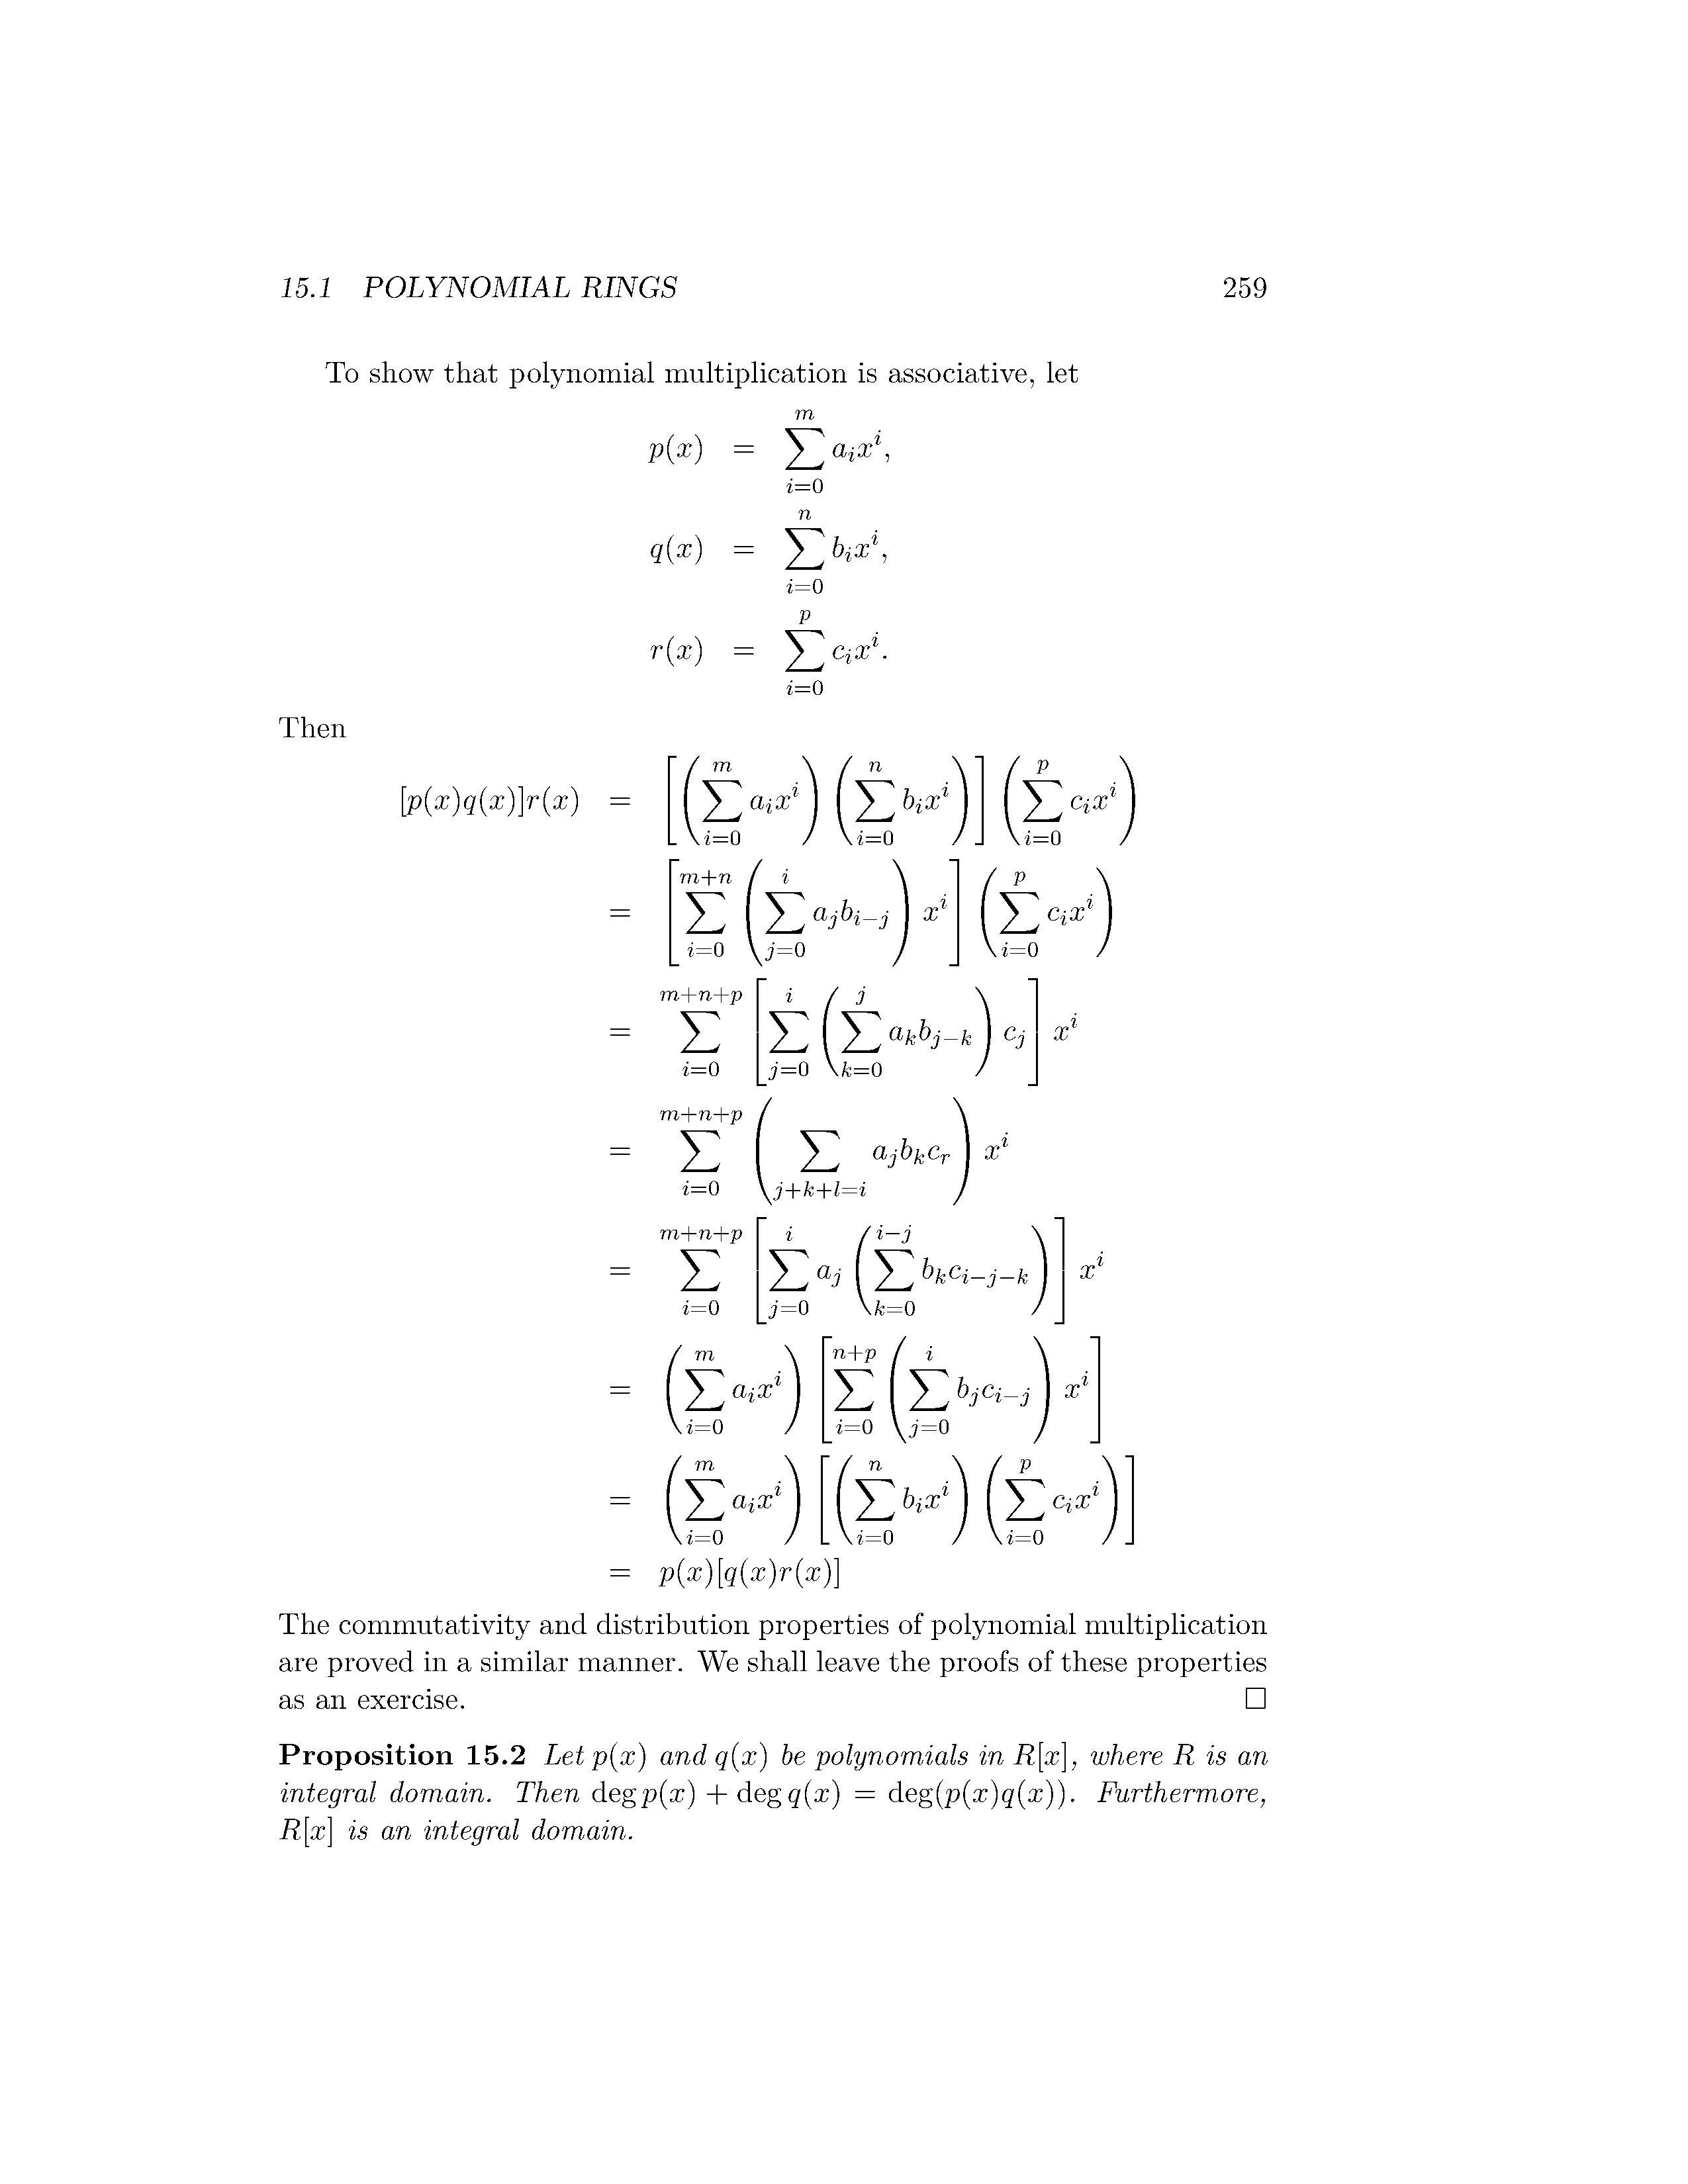
\includegraphics[width=1.0in, height=1.3in]{org.png} &
 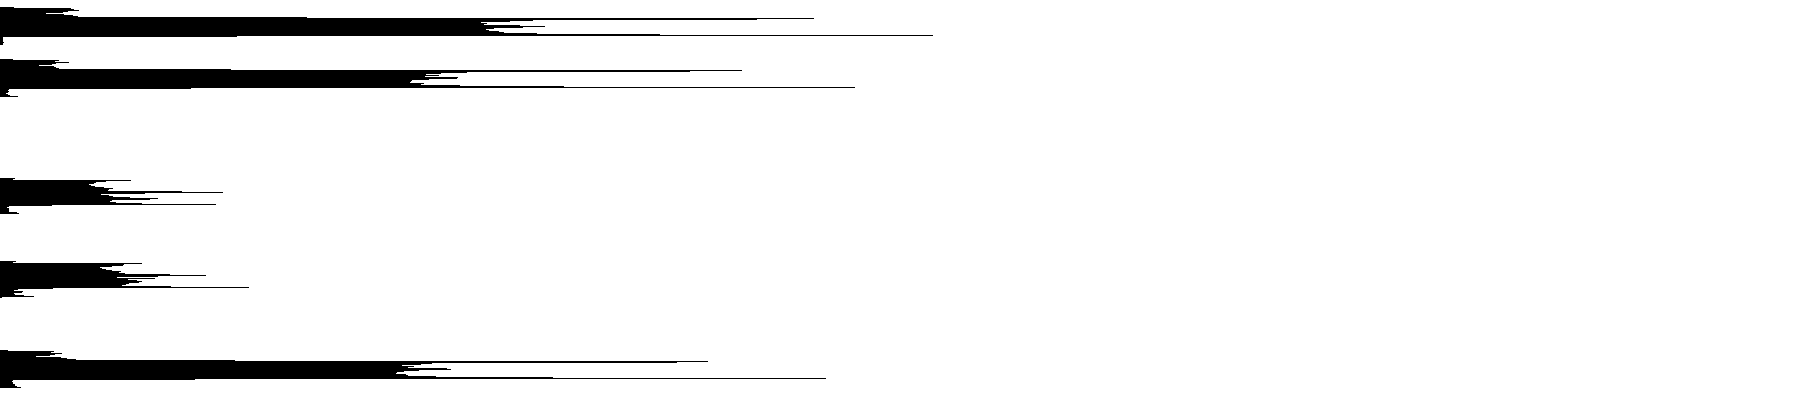
\includegraphics[width=0.8in, height=1.3in]{hProj.png} \\ 
 (a) Image &(b) Horizontal Projection Profile
 \\\hline
 \end{tabular}
 \caption{A document page and its horizontal projection profile}
 \label{hproj}
\end{figure}
 
 
 \item[2.] {\em Creation of word blobs in Text lines}\\
 This is done by merging the characters in a word. Such character coalescing process depends on the accuracy in detecting the normal
character gap and the gap between the consecutive connected components in that text line.

The mathematical formulation for  blob formation is as follows.
Consider a binary image $I_{P \times Q}$, which consists of connected
components $C_k (k=1,2,\ldots ,P)$, as defined in standard text \cite{gonzalez92}
with their usual meanings.
Let $L(C_k)$, $R(C_k)$, $T(C_k)$ and $B(C_k)$
be the four corner  points of the $k_{th}$ connected component in  left, right, top and bottom
directions respectively.

\begin{figure}[h]\center\footnotesize
\begin{tabular}{|c|c|}\hline
 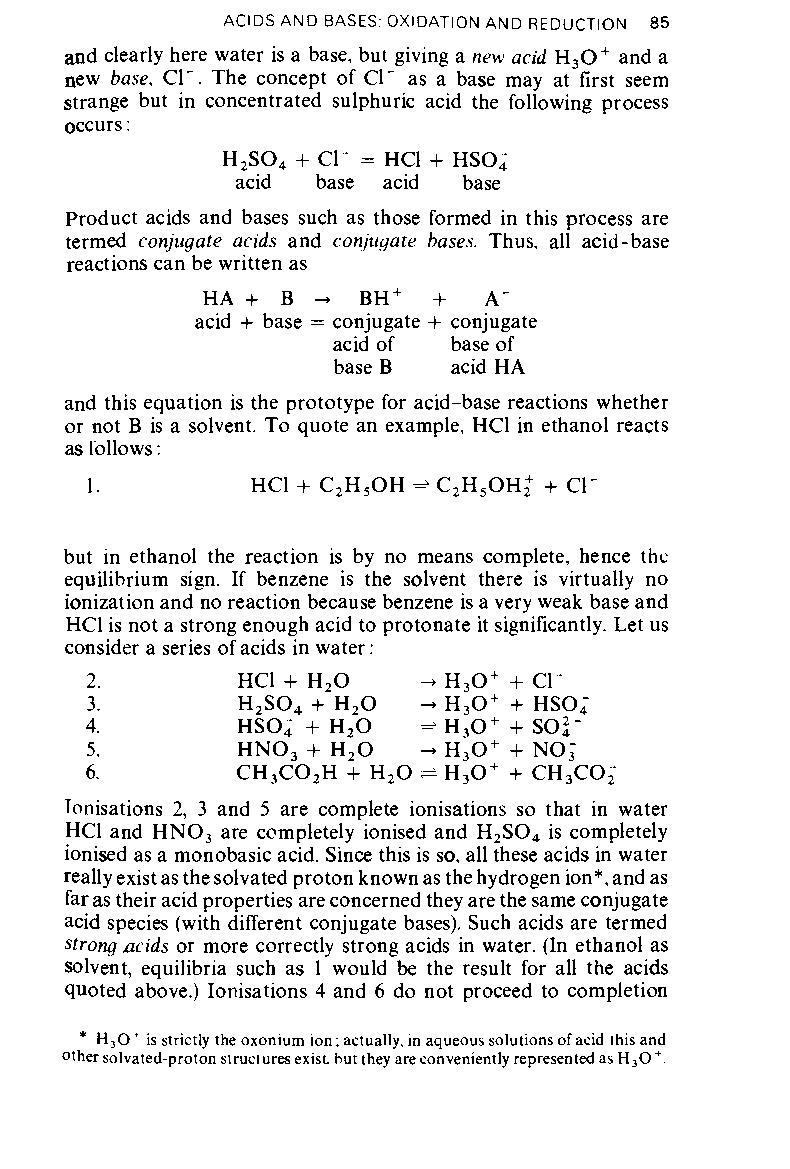
\includegraphics[width=1.0in, height = 1.2in]{page_image.png} &
 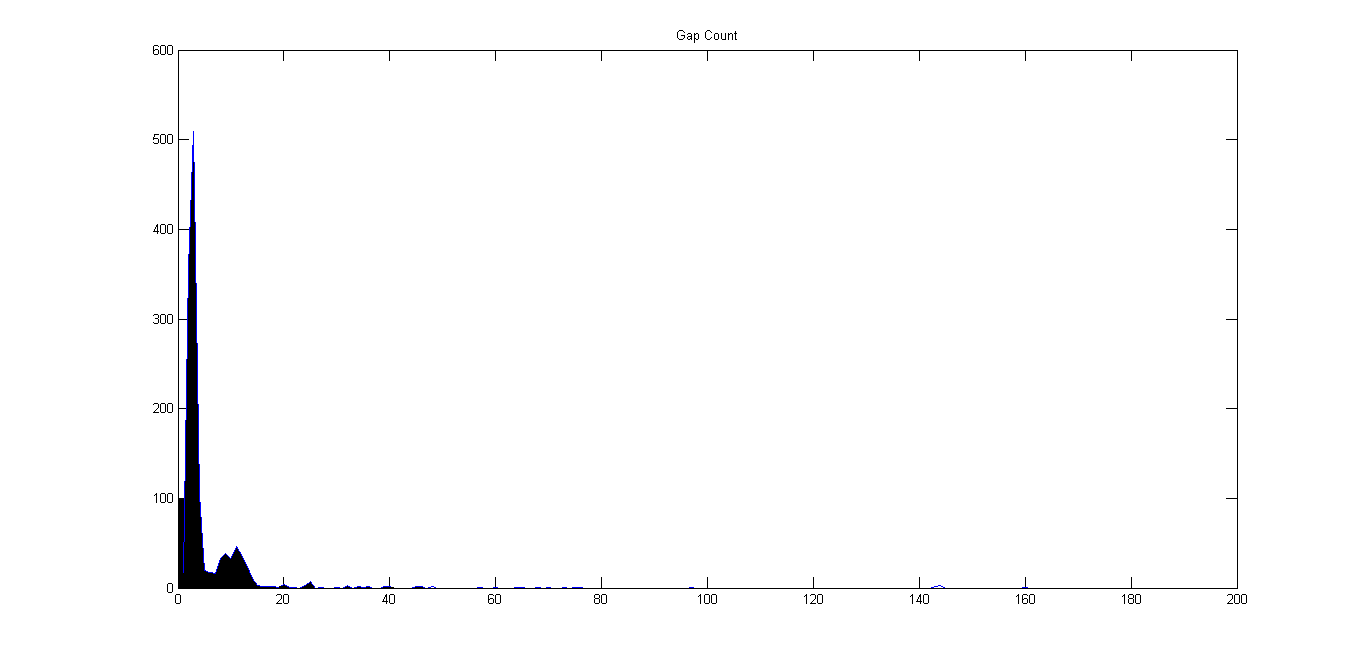
\includegraphics[width=0.25\textwidth]{cw_gap.png} \\ 
 (a)  &(b)
 \\\hline
 \end{tabular}
 \caption{Example of a page and histogram. (a) Document page (b) Histogram of the preprocessed page.}
 \label{page_histo}
\end{figure}

Let  $F$ be a function which ensures that the two connected
components lie in the same text line.
Then $F$ may be represented as
{\scriptsize
\[F(C_a,C_b)=\left\{ \begin{array}{llc}
1 & \mbox{if} & (T(C_a)\leq B(C_b)\  AND\  B(C_a)\geq T(C_b)) \\
0  & \multicolumn{2}{l}{\mbox{otherwise}}
\end{array} \right. \]
}

Cluster formation requires information on inter-word gap. 
%This may be  obtained
%from  the histogram $H_1$ of the distance $D$ between two consecutive connected components $C_a$
%and $C_b$ as follows.

The  distance function, D, obtained from the histogram $H_1$, is defined for computing the horizontal
distance between any two consecutive connected components $C_a$ and $C_b$, as shown below
\[D(C_a,C_b) = L(C_b) - R(C_a)\]
where $b = \min\limits_x$\{${ L(C_x) - R(C_a)}$\} such that $(F(C_a,C_x) = 1$
AND $L(C_x)>R(C_a))$.
The histogram $H_1$ registers the  gap between
two consecutive characters.
It may be noted that  there may be more than two
distinct humps in $H_1$, first one represents the character gaps in  words and the second one
represents the normal word gaps in  text lines. An example page
and corresponding histogram is shown in
Fig.~\ref{page_histo}(a) and (b).

\begin{figure}[h]\center\footnotesize
 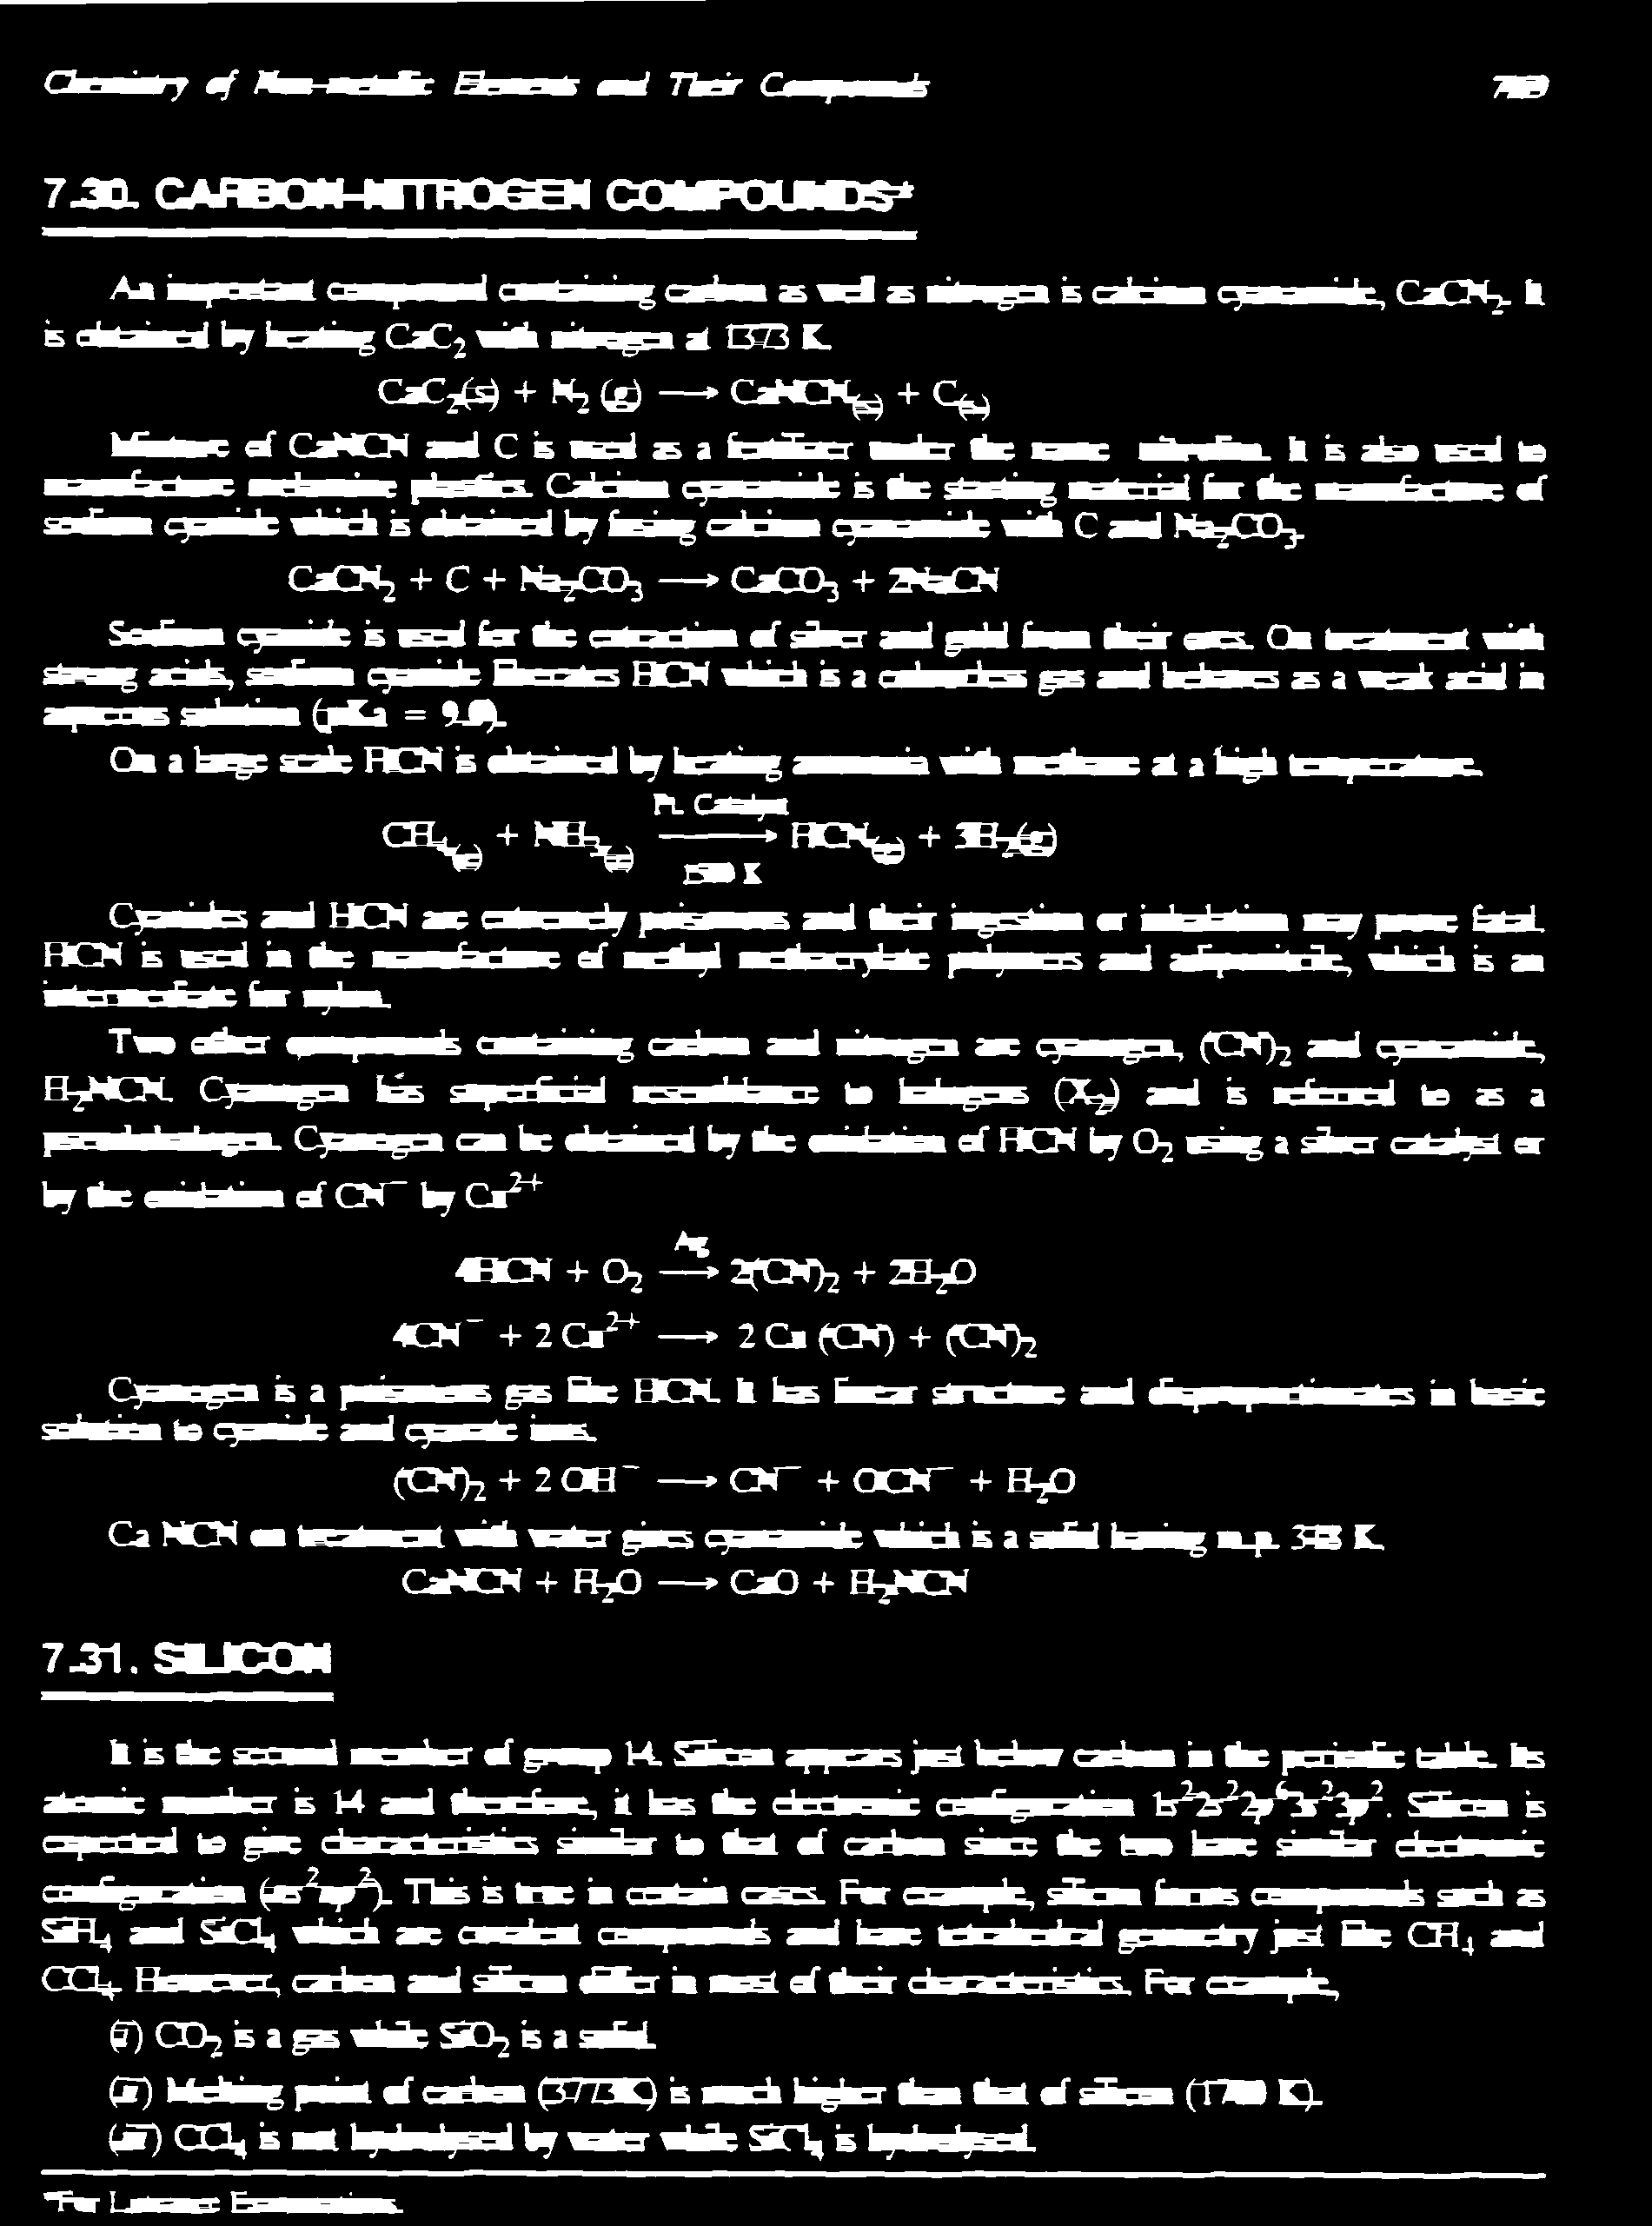
\includegraphics[width=0.4\textwidth]{wordBlob.png} 
  \caption{Example of blob formation. Clusters formed from a portion of the image shown in
Fig.~\ref{page_histo}(a).}
 \label{word_blob}
\end{figure}


%\begin{table}[h]\center\scriptsize
%\caption{ Operators and their features}
%\begin{tabular}{|l|c|c|c|}\hline
                   
%Operators            & horizontal project  & vertical projection & ratio of height and width  \\ \hline
 % + & one peak at the center & one peak at the center & 1\\ \hline
  %- & one peak with width & flat & $\leq 3/5$ \\
   % &is equal to the width & & \\ 
    %&of the component &  &\\ \hline
  %$\times$ & two humps  & two humps & $\simeq  1$\\  
  % & separated by &separated by &\\
   %& a small valley & a small valley & \\ \hline
  %$\sum$ & two peaks with  & two humps & $ > 1$\\
  %& equal height &at two ends & \\
  %& at two ends & & \\ \hline
  %$\prod$& two unequal peaks & two equal peaks  & $ > 1$\\
   %  & at two ends & at two ends & \\ \hline
%\end{tabular}
%\label{tab:summary}
%\end{table}

Our intention is to
find out character gaps in running texts of a document page so that we could
combine the consecutive characters into a single blob. Hence, we consider
the upper boundary ($\upsilon$) of the first hump as the length of structuring
element. Morphological
close operation with a structuring element of area
$\ (\upsilon \times \ 1)$ will form the blobs denoted as
$V_w$ (where $w\ =\ 1,2,\ldots ,Q$). The
blob formation will be dictated by the following
two conditions:
\begin{enumerate}
\item If there are two connected components $C_m$ and $C_n$ $\ (1\leq m,n\leq P)\ $
obeying the relations
\begin{itemize}
\item $ \ F(C_m, C_n) = 1 $
\item $ D(C_m, C_n) \leq \upsilon $
\end{itemize}
then $C_m$ and $C_n$ should belong to the same blob.
\item $ V_a \cap V_b = \emptyset \ \ \forall \ a,b \ | \ (1\leq (a,b) \leq Q \ \ AND \ \
 a \not= b)$
\end{enumerate}


\item[3.] {Operator  identification}\\
\label{op_id}
We have considered the set of operators that is commonly used both in  chemical equations as well as mathematical 
equations to fulfil our aim to classify displayed zones containing chemical and non-chemical equations.

\begin{figure}[htb]\center\footnotesize
\begin{tabular}{|c|c|c|}
\hline
Operators & horizontal projection & vertical projection\\ \hline

\includegraphics[width=0.2in, height=0.2in]{plus.png} &
 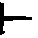
\includegraphics[width=0.2in,height=0.2in ]{plusH.png} & 

\includegraphics[width=0.2in,height=0.2in]{plusV.png}\\ \hline

\includegraphics[width=0.2in, height=0.02in]{minus.png} &
 
\includegraphics[width=0.2in,height=0.02in ]{minusH.png} & 

\includegraphics[width=0.2in,height=0.02in]{minusV.png}\\ \hline
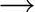
\includegraphics[width=0.2in, height=0.05in]{arrow.png} &
 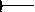
\includegraphics[width=0.2in,height=0.05in ]{arrowH.png} & 

\includegraphics[width=0.2in,height=0.05in]{arrowV.png}\\ \hline
%
\includegraphics[width=0.2in, height=0.2in]{sigma.png} &
 %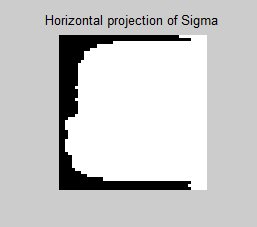
\includegraphics[width=0.2in,height=0.2in ]{sigmaH.png} & 
%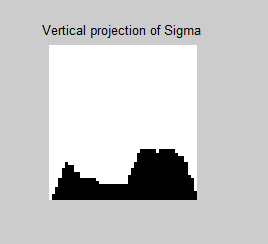
\includegraphics[width=0.2in,height=0.2in]{sigmaV.png}\\ \hline
%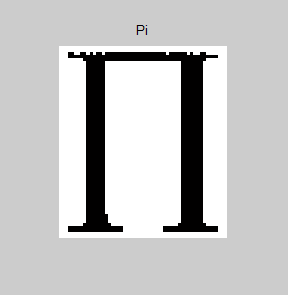
\includegraphics[width=0.2in, height=0.2in]{pi.png} &
 %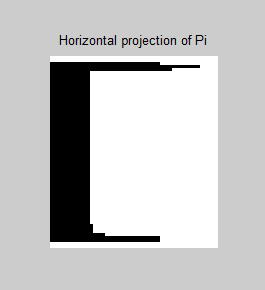
\includegraphics[width=0.2in,height=0.2in ]{piH.png} & 
%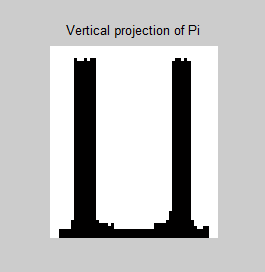
\includegraphics[width=0.2in,height=0.2in]{piV.png}\\ \hline
\end{tabular} 
 \caption{Operators and their horizontal and vertical projection profiles}
 \label{h_v_profile}
\end{figure}
\begin{figure}[h]\center\footnotesize
\begin{tabular}{|c|}\hline
 
\includegraphics[width=0.42\textwidth]{singleChar.png} \\\hline
 \end{tabular} 
 \caption{Sigle components extracted from the word blobs shown in Fig.~\ref{word_blob}}
 \label{single_char}
\end{figure}

\begin{figure}[h]\center\footnotesize
\begin{tabular}{|c|}\hline
 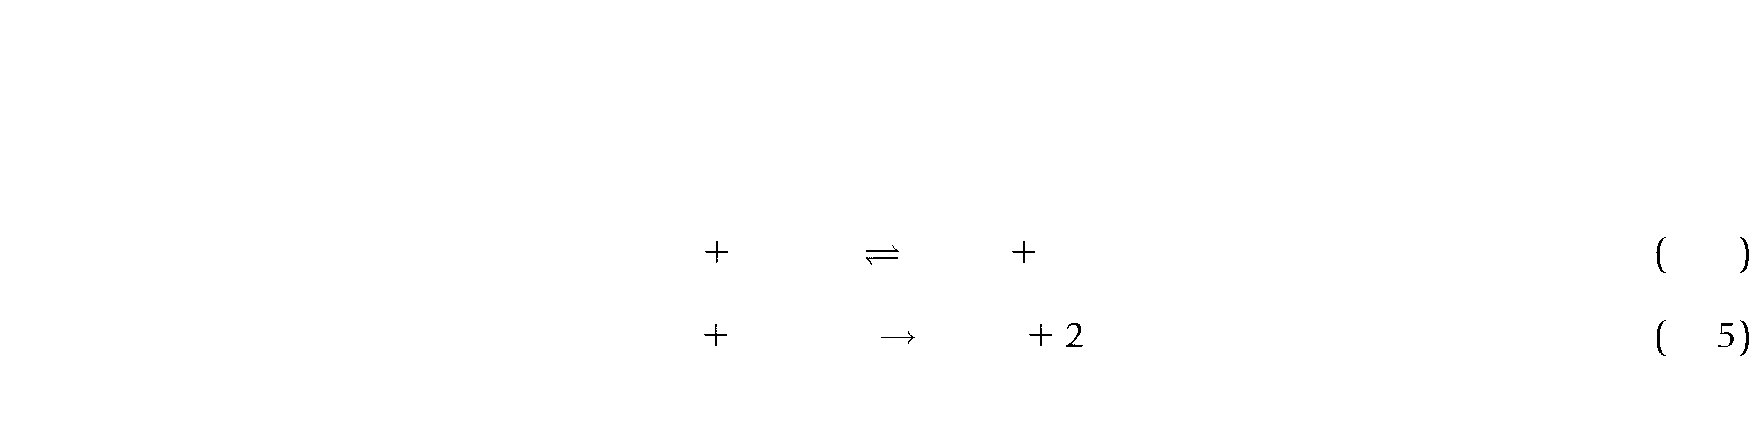
\includegraphics[width=0.42\textwidth]{singleCharafterEuler.png} \\\hline
 \end{tabular} 
 \caption{After removal of alphanumerals based on Euler number from the image shown
in Fig.~\ref{single_char}}
 \label{after_euler}
\end{figure}

\begin{figure}[h]\center\footnotesize
\begin{tabular}{|c|}\hline
 
\includegraphics[width=0.4\textwidth]{operator.png} \\\hline
 \end{tabular} 
 \caption{Operators extraceted from the image shown in Fig.~\ref{after_euler}}
 \label{operator}
\end{figure}

After blob formation, each blob is labeled. The region corresponding to each blob is considered from
the original image and the number of connected component present in that region is counted. If the number of components
is more than one that blob is not an operator and is removed from the blob image (see. Fig.~\ref{single_char}).
The remaining components in the blob image are operators along with some alphanumerics like 'a', 'A', '(' etc.
The logical AND operation is performed between the blob image and the original image. 
The Euler number of the operators
that we have considered is 1 and based on this feature some of the alphanumerics are discarded (see Fig.~\ref{after_euler}).
This image is denoted by the name $I_{singleChar}$.
We then extracted the following features:\\
\begin{itemize}
 \item Aspect ratio ($f_a$) of each component
 \item 
 Density \[f_d   = \frac{\#pixels_o} {\#pixels_b}, \]
 where $\#pixels_o$ denotes the number of object pixels and $\#pixels_b$ denotes area of the bounding box.
 \item Each component is resized and horizontal and vertical projection profiles (see Fig.~\ref{h_v_profile})  are obtained.\\
 (i) For each profile the second ($f_{m2}$) and third moments ($f_{m3}$) are calculated. \\
 (ii) Again for each profile the location($f_l$) and the magnitude ($f_m$) of the global maximum are determined.
 \item Perimeter ($f_p$)  of each component is also obtained.
\end{itemize}

Now, [$f_a,f_d,f_{m2}^h,f_{m2}^v,f_{m3}^h,f_{m3}^v,f_l^h,f_l^v,f_m^h,f_m^v,f_p$] serve as the feature descriptor for classification of operators from 
$I_{singleChar}$. An $one$-$class$ SVM is used to classify the single components into two classes - operators (+,-,$\leftharpoondown$,$\rightharpoonup$,$\rightarrow$,$\leftrightarrow$)
and non-operators (all remaining single characters). In case of $multi$-$class$ SVM total number of classes to be considered would be more than 62 (including alphanumerics, operators etc.).
Hence, $one$-$class$ SVM is more suitable according to our requirements. The accuracy of the classifier is 98.4\% 

%The project profiles for the operators are shown in Fig.~\ref{h_v_profile} and it is observed from the
%figure that each operator has its unique horizontal and vertical project profiles. 
%The horizontal and vertical projection profiles are resized and the second order and third order moments
%are obtained for each projection profile. The moments and the aspect ration are used to identify the
%required operators. 
%%% SVM must be discussed.
%These features are used to recognize  the operators (see Fig.~\ref{single_char}(c)).
% The rightarrow which is common in chamical equations is identified as minus.
To detect `=' or `$\rightleftharpoons$' one extra step is required. 
The operators having $f_a$ $\leq$ 0.6 are considered to be thin symbols (-,$\leftharpoondown$,$\rightharpoonup$,$\rightarrow$,$\leftrightarrow$). 
 For each symbol denoting thin operator, a rectangular mask is placed below the
symbol to check if there is another one within the mask; if present the two thin operators are considered to form
an `=' or `$\rightleftharpoons$' sign. Let the length of the thin operator be $l$. The area of the  mask is  ($l \times l/2$).\\

The horizontal line separating  the numerator and the denominator is identified by its length which is greater than
the median length of the operators. Two windows are placed above and below  the separating line to merge all
the components within the windows with the separating line to form a single logical line. Otherwise, they would be
treated as three consecutive text lines and we will not be able to associate the intermediate math-symbols (`+', `-', `=')
 to a single expression. The area of the window is (length of the separating line) $\times$ (twice the median height of the text
lines).


\item[4.]{Segmentation of DE zones}\\
Initially, all the text lines consisting of at least one operator are considered as candidate displayed equations (CDE).
The operators are eliminated from CDE. The upper boundary ($u_v$) of the second hump of the histogram $H_1$ is obtained
which represents the word gaps in the text line. For each CDE zone Run Length Smoothing Algorithm  in horizontal direction (  H-RLSA) is 
carried out. If the distance between two neighbouring
components is less than $u_v$, it means they belong to a same word and thus are merged by H-RLSA.
H-RLSA has a similar effect as of dilation of black areas in horizontal direction. The characters
in a word are dilated and get linked/connected to the other characters of the same word. The output of
H-RLSA is shown in Fig.~\ref{h-rlsa}.
% 
% \begin{figure}[h]\center\footnotesize
% \begin{tabular}{|c|c|c|}
% \hline
%  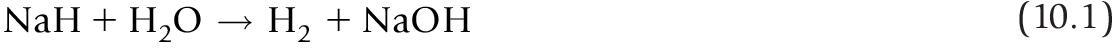
\includegraphics[width=2.4in, height=0.1in]{line.png} &
%  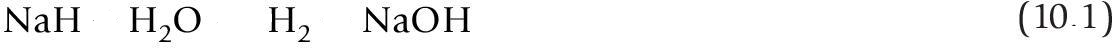
\includegraphics[width=2.4in, height=0.1in]{linewithoutOP.png} &
%  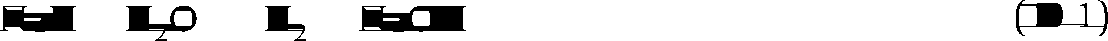
\includegraphics[width=2.4in, height=0.1in]{lineClosed.png}\\ 
%  (a)   & (b) &(c) \\\hline
%  \end{tabular} 
%  \caption{The output of H-RLSA on portion of an image (a) a part of an image;
%  (b) same part without operators; (c) result of H-RLSA operation }
%  \label{h-rlsa}
% \end{figure}


\begin{figure}[h]\center\footnotesize
\begin{tabular}{|c|}
\hline
 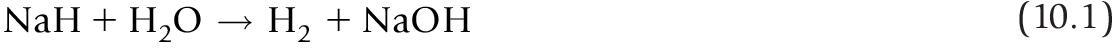
\includegraphics[width=0.4\textwidth]{line.png} \\
 (a)\\ \hline
 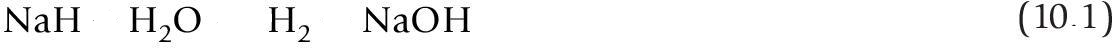
\includegraphics[width=0.4\textwidth]{linewithoutOP.png} \\
 (b) \\ \hline
 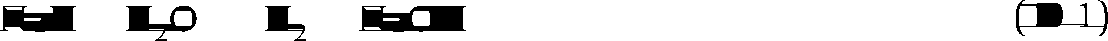
\includegraphics[width=0.4\textwidth]{lineClosed.png}\\ 
 (c) \\\hline
 \end{tabular} 
 \caption{The output of H-RLSA on portion of an image (a) a part of an image;
 (b) same part without operators; (c) result of H-RLSA operation }
 \label{h-rlsa}
\end{figure}

The equation number is common in the displayed equation zone. This has to be removed because for each CDE
we have counted the number of operators  and corresponding other components  in the output of H-RLSA. If the number of components 
 $\le$ 2$\times$ number of operators, then the CDE is considered as a displayed equation;
otherwise some embedded formulas/equations may exist in the line. To eliminate the equation number from the output of H-RLSA  the operators are  moved here and the component 
analysis is done. From both ends distance ($d$) (see Fig.\ref{end_rev})between the first two consecutive components is measured and if $d$  $> 5\times$  $u_v$, 
then the first component from the end is considered as equation number and is removed.
\begin{figure}[h]\center\footnotesize
\begin{tabular}{|c|}
\hline
 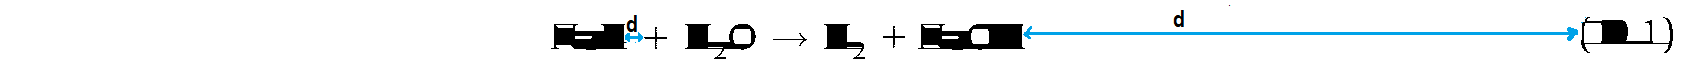
\includegraphics[width=0.41\textwidth]{endRemoval.png} \\ \hline
 \end{tabular} 
 \caption{Example of a equation number present in DE zone}
 \label{end_rev}
\end{figure}
\item[5.]{Classification of segmented DE zones}\\
Each segmented displayed equation is divided into three zones; namely upper zone, middle zone and lower zone (see Fig~\ref{sub_super}).
To identify the three zones of a DE zone, uppermost and lowermost co-ordinates of each connected component below the same DE zone  are also obtained.
The median of uppermost coordinate, and median of lowermost co-ordinate of such components in DE zone are computed.
A horizontal line, called the baseline, is drawn through the median of lowermost coordinates of components
and this baseline separates the middle zone and lower zone of DE zone.
Similarly, the median of uppermost co-ordinate of the components in the DE zone  generates a horizontal line. This horizontal line, called top line, separates the middle and  upper zones of the DE zone.
\begin{figure}[h]\center\footnotesize
\begin{tabular}{|c|}
\hline
 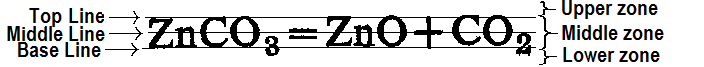
\includegraphics[width=0.32\textwidth]{s_s.png} \\ \hline
 \end{tabular} 
 \caption{Example of 3 zones present in a DE zone}
 \label{sub_super}
\end{figure}


The subscripts in a DE zone belong to lower-half of the middle zone and lower zone whereas the superscripts belong to upper zone and
upper-half of the middle zone. Based on the location of the components in a DE zone we have detected the subscripts and superscripts
and removed from the DE zone. The operators are also removed from DE zone.

Now, each displayed equation is an input of  an OCR engine, Google Tesseract 3.02.
The OCR returns each DE zone as a text string.
We made a dictionary out of all the elements in the periodic table. An important observation is that an element always starts with a capital letter. Using this property,
an element can be expressed by a regular expression [A-Z][a-z]*. 
It means an element's symbol
starts with an upper case letter and may or may not have one or more lower case letters. 
We have designed a parser to extract the sub-strings matching the above-mentioned regular expression with the following grammar:\\
\begin{center}
$start \rightarrow capital.follow$\\
$follow \rightarrow small.follow | \in$\\
$capital \rightarrow A|B| \dots |X|Y|Z$\\
$small \rightarrow a|b| \dots |x|y|z$\\
\end{center}

The working principle of the parser is depicted in Fig.~\ref{flow_chart}.
Each of the substrings returned by the parser is matched against the aforesaid dictionary and if it is a positive match then 
that substring is considered as a symbol of the chemical element. 
Let us consider, the number of substrings extracted from the OCR output by the parser is {\em n}  and the number of positive matches with 
the aforementioned dictionary is {\em m}.
If m:n ratio is more than a threshold value $\beta$ then this DE is considered as a Chemical Equation. 
This threshold ($\beta$) is set to 0.7 by running our algorithm on our dataset containing 733 segmented displayed equations. 
The reasons for $\beta$ not being 1 are
i) limitation of the OCR we used;
ii) presence of broken and touching characters in the DE zone.

\begin{figure}[h]\center\footnotesize
\begin{tabular}{|c|}
\hline
 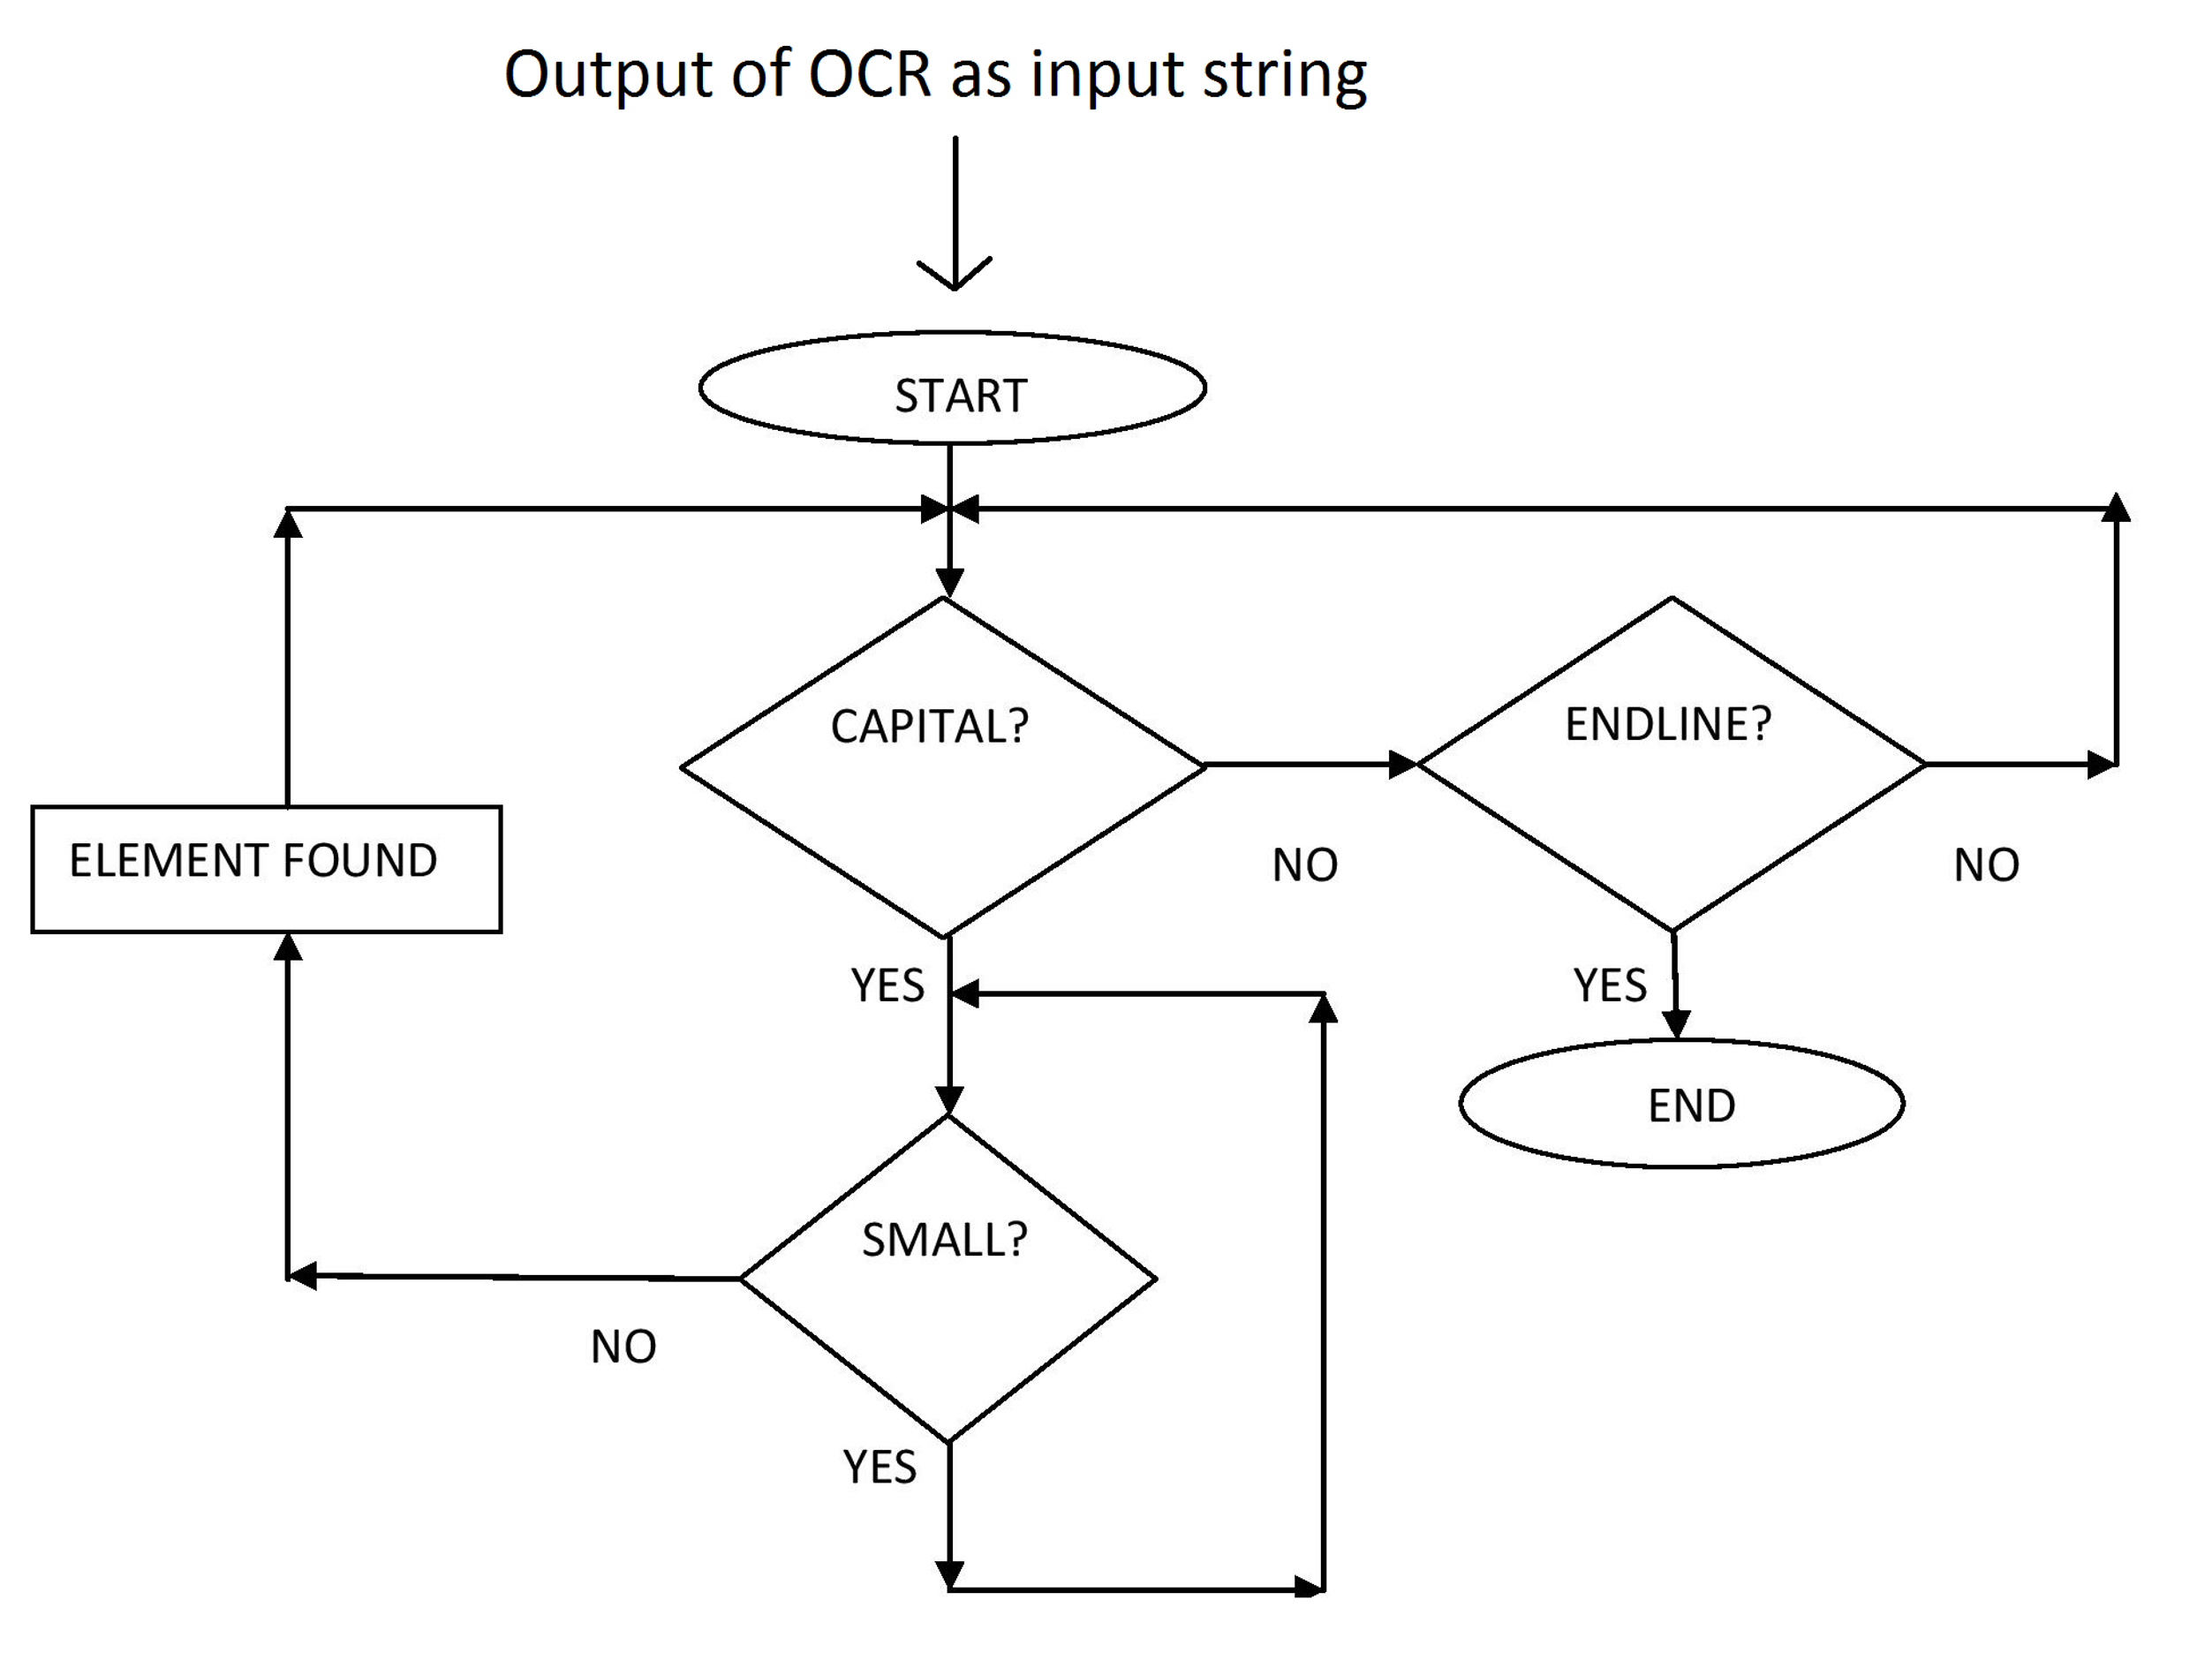
\includegraphics[width=0.35\textwidth]{flowchart.png} \\ \hline
 \end{tabular} 
 \caption{Working flow chart of the parser}
 \label{flow_chart}
\end{figure}
\end{itemize}

\section{Experimental Result}
\label{sc_exp_res}
We have implemented our algorithm in MATLAB 8.3.0.532 (R2014a) in a PC (Intel core 2 Duo T6500 2.1\,GHz CPU running Windows 8).
The proposed method has been tested  on a dataset consisting 152 document pages. Out of 152 pages 50 pages are taken from
ICDAR 2013 Math-zone segmentation datasets and other document pages are scanned from different Chemistry books.
Altogether 752 displayed equations are spotted manually from the dataset. Our method segmented
733 DE zones from the dataset which is manually verified.  Our method is not applicabe for segmentation of some of the
displayed math-zones like conditional equations and matrices because our motivation is to classify the chemical and non-chemical
equations.  The results (see Table 1)
show a high degree of accuracy and low mis-classification
percentage for both chemical and non-chemical expressions obtained from our dataset.
 Classification outputs for some of the cases are shown in Fig.~\ref{exp_result}. In the figure  the  red and the green bounding boxes indicate chemical and 
non-chemical expressions respectively.

\begin{table}[h]\center\scriptsize
\caption{ Summary of experimental results}
\begin{tabular}{|l|c|c|c|}\hline
                   
%$\frac{Classified as}{ Actual}  $           & Chemical & Otherl \\ \hline
%\diagdown{Classified as}{ Actual}          & Chemical & Otherl \\ \hline
%Chemical & 97.8\% & 2.2\%\\ \hline
%Non-chemical & 2.95\% & 97.05\%\\ \hline

\diaghead{\theadfont tableOfExperiment}%
{Actual}{Classified\\As}&
\thead{Chemical}&\thead{Other}\\ \hline
Chemical & 97.8\% & 2.2\%\\ \hline
Other & 2.95\% & 97.05\%\\ \hline

\end{tabular}
\label{tab:summary}
\end{table}

\begin{figure*}[h]\center\footnotesize
\begin{tabular}{|c|c|}
\hline
 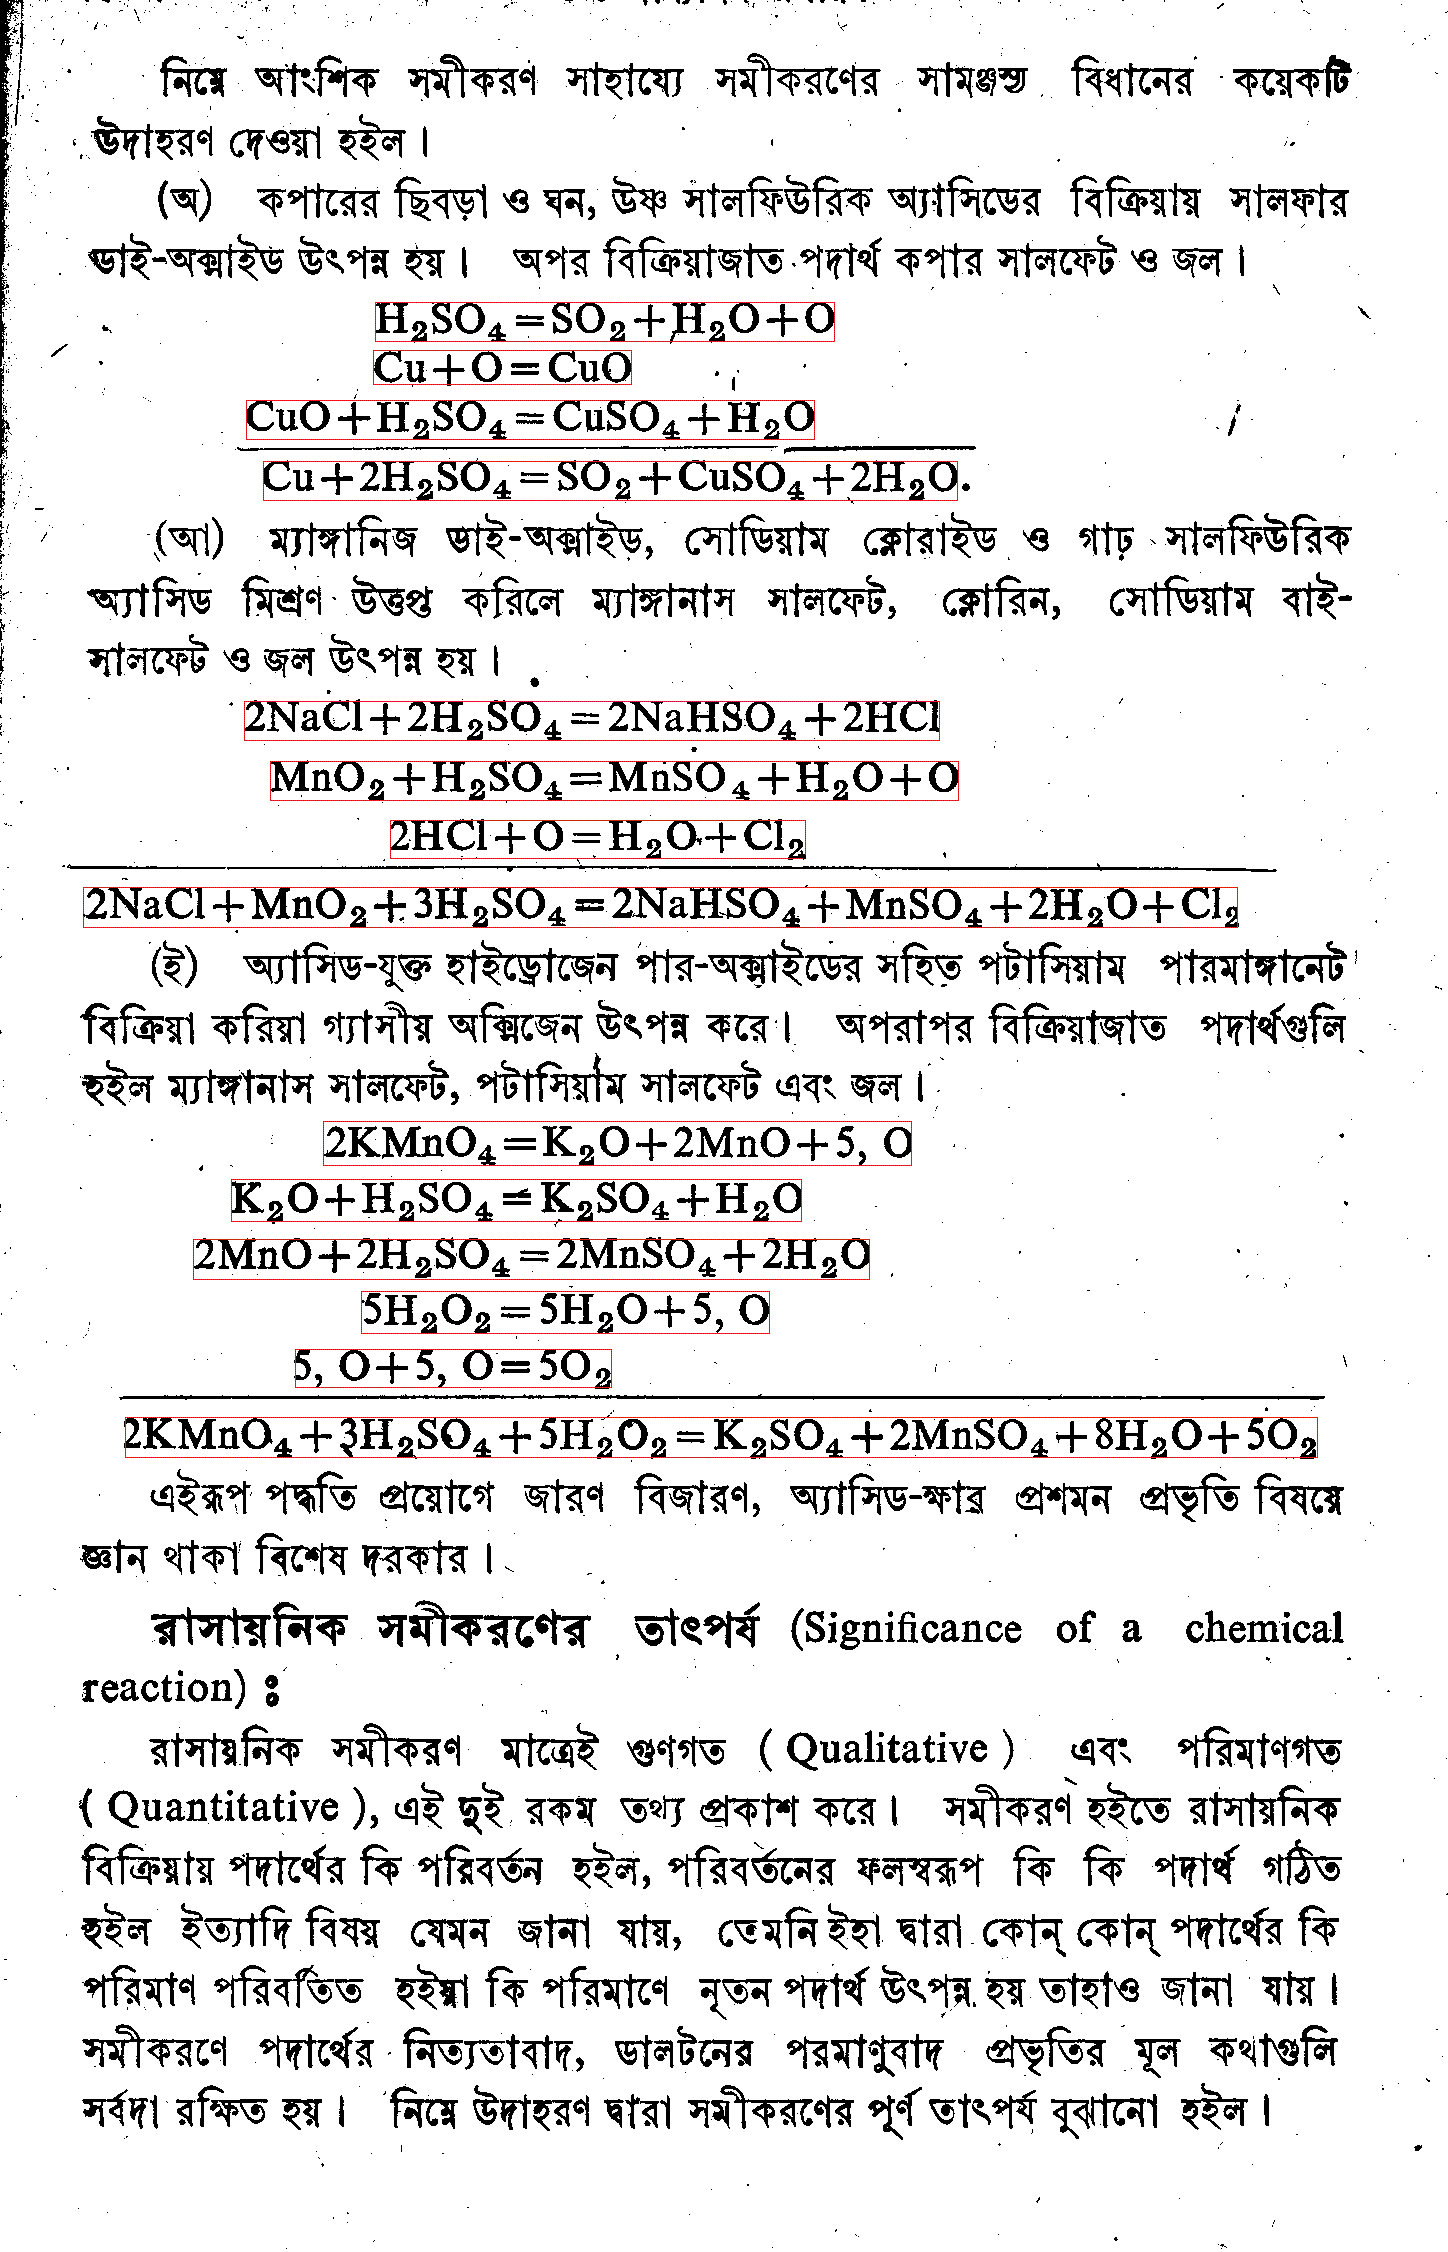
\includegraphics[width=0.42\textwidth]{result1.png} &
 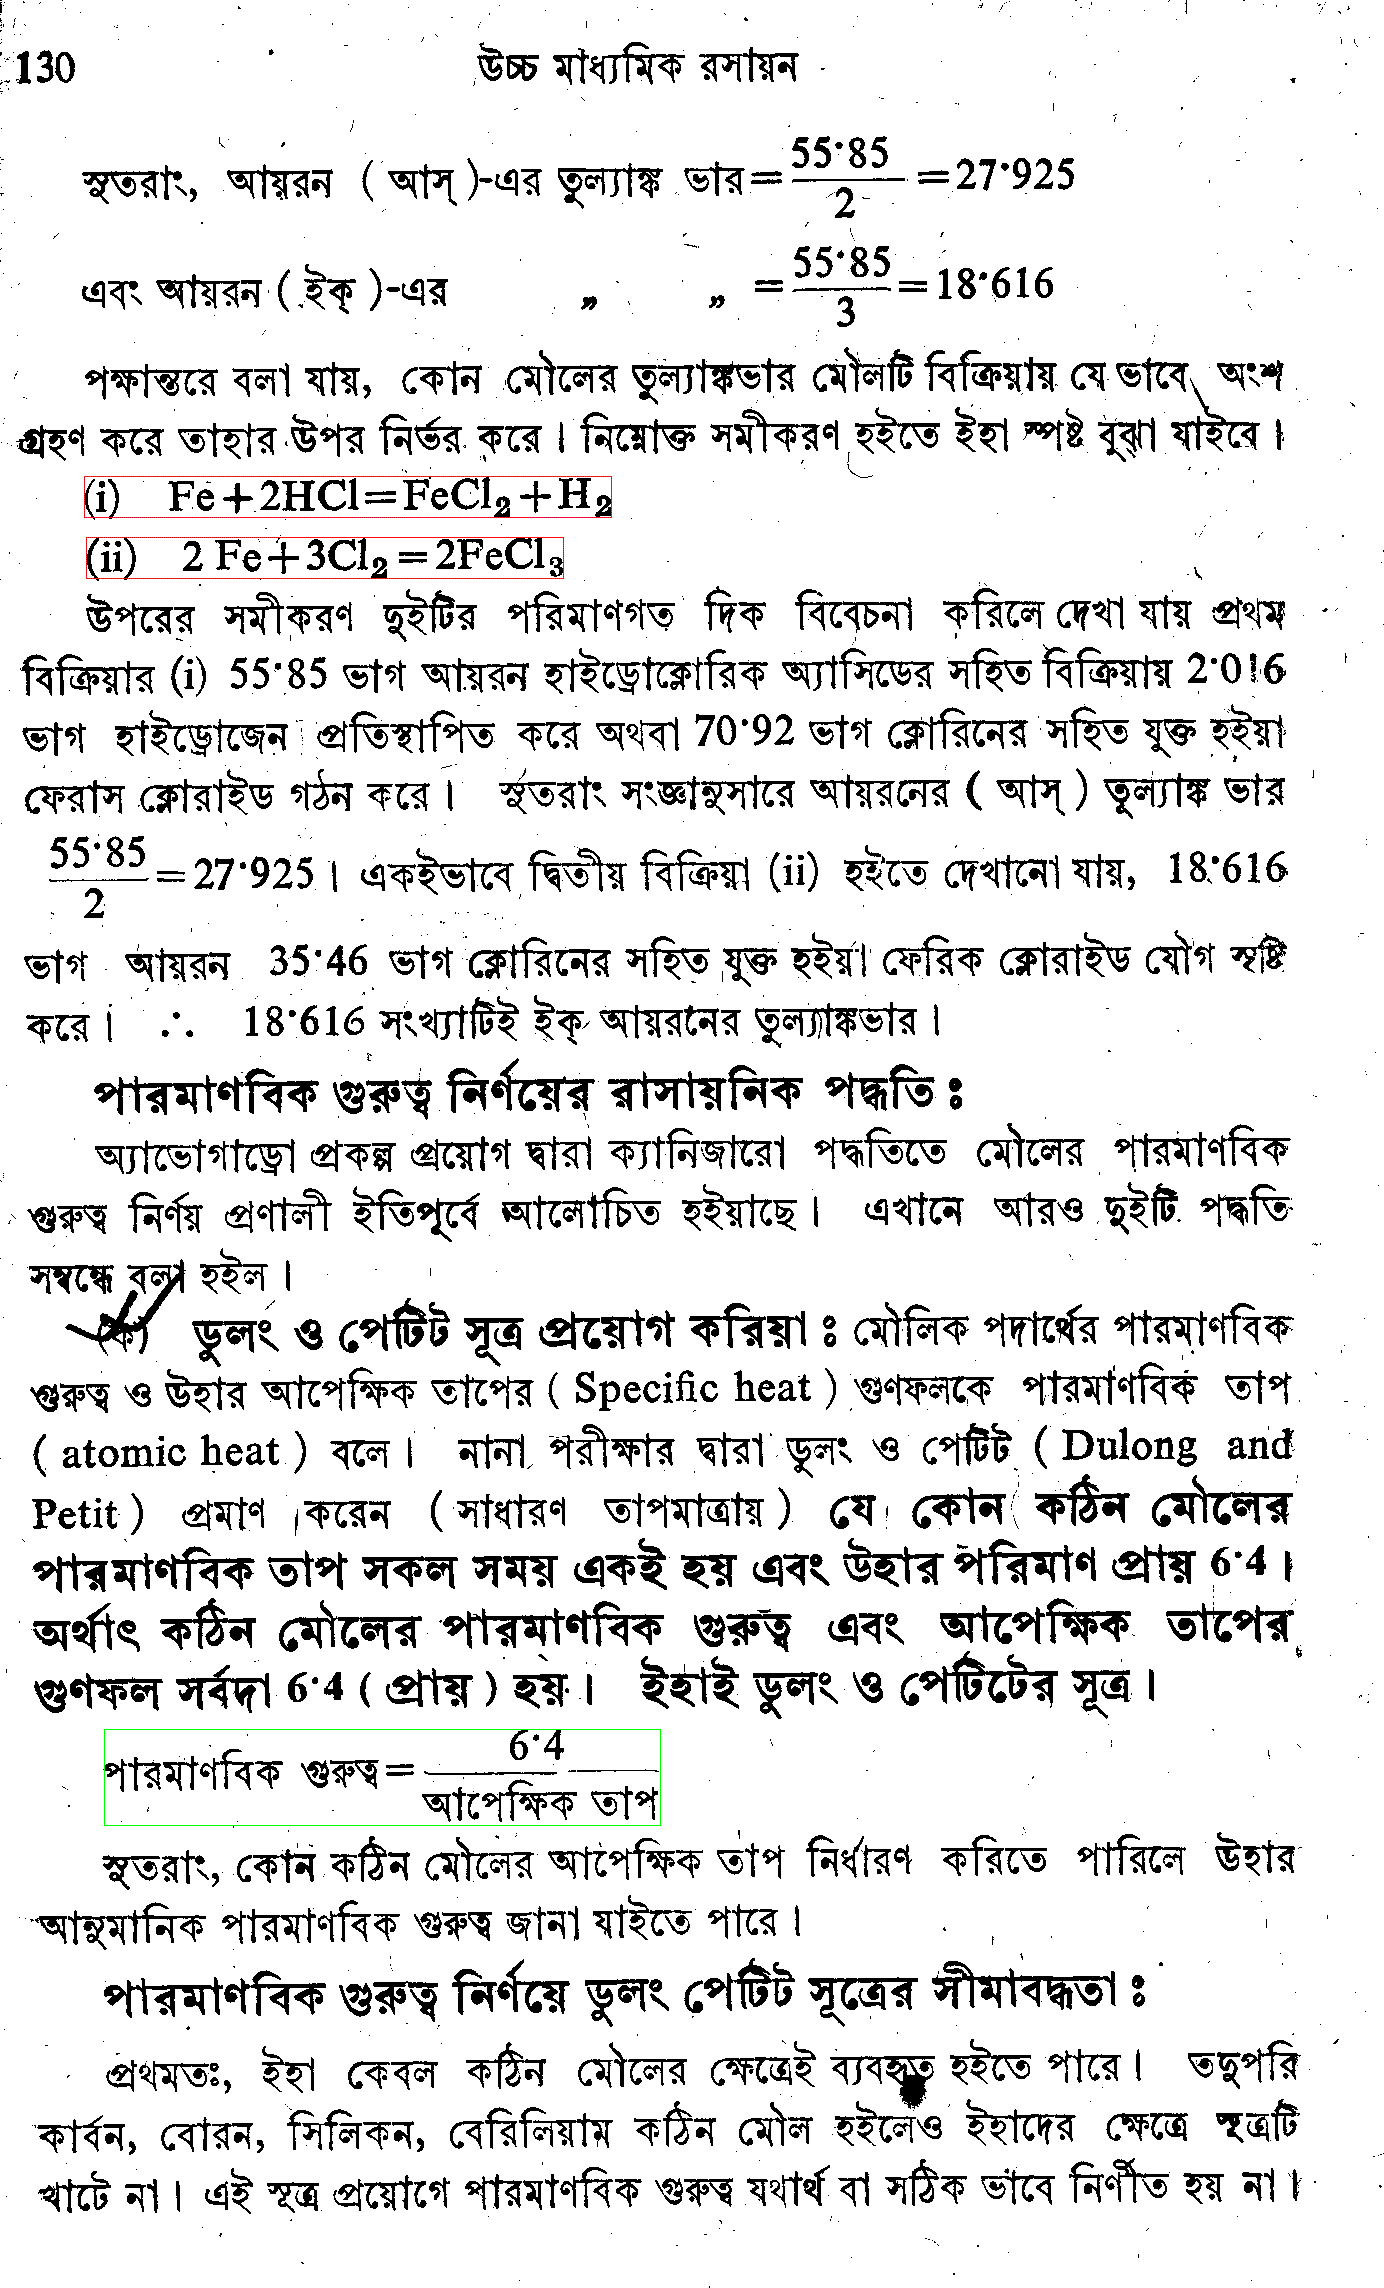
\includegraphics[width=0.42\textwidth]{result2.png} \\
 (a)  &(b)  \\
 \hline
  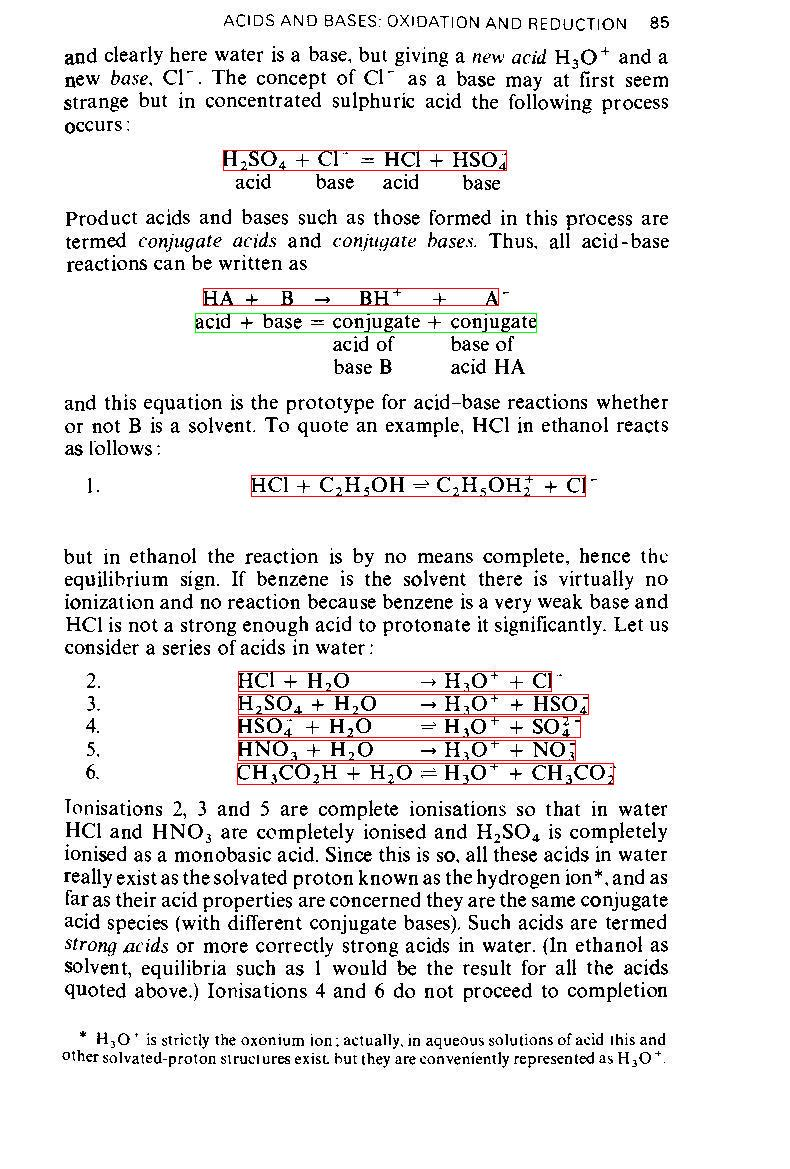
\includegraphics[width=0.42\textwidth]{result_3.png} &
 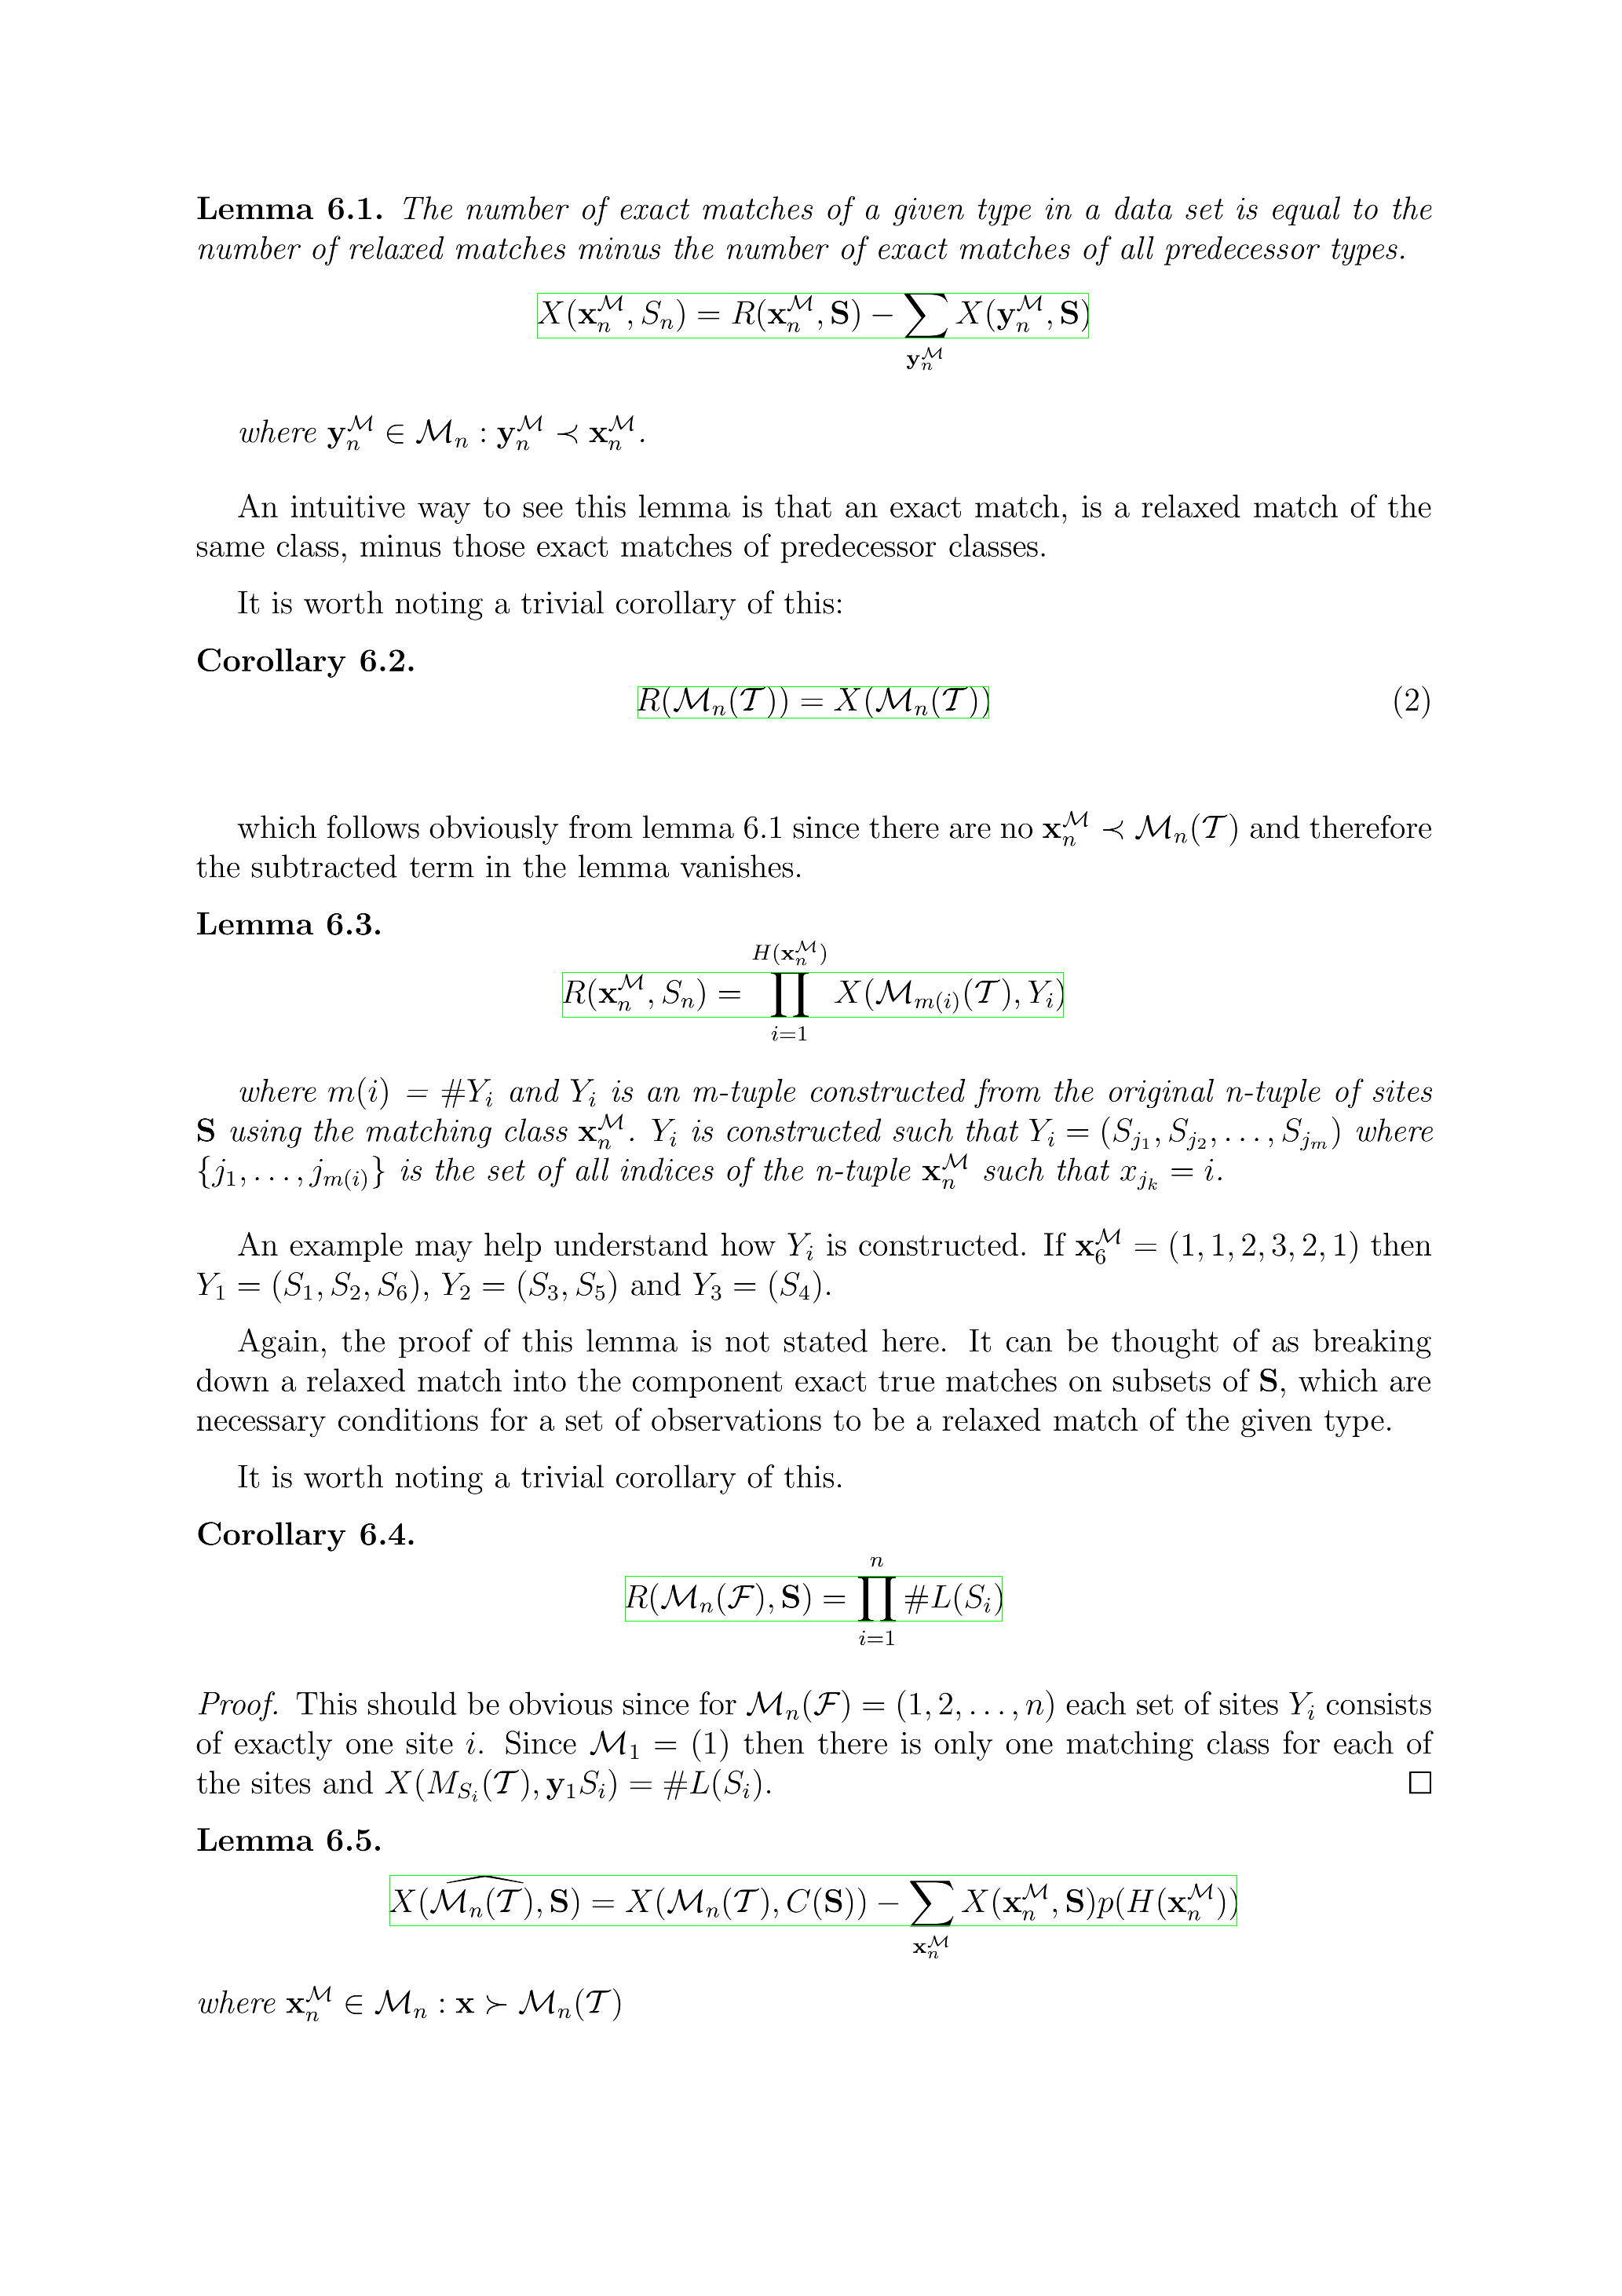
\includegraphics[width=0.42\textwidth]{result4.png} \\
 (c)  &(d)  \\
 \hline
 \end{tabular} 
 \caption{Samples of classification result }
 \label{exp_result}
\end{figure*}


\subsection{Error Analysis}
Here we try to analyse the sources of some of the errors which have negative effect on the performance figures both for segmentation and classification.
\begin{itemize}
 \item Segmentation error:\\
 %Cosider the Fig.~\ref{seg_error} 
 
 Some chemical equations have some reactants/symbols (such as $\Delta$) just on top or bottom of the arrow   
 and in some cases they enter the bounding box of the arrow.  
  When we extract only single characters from the word blob information as mentioned in ~\ref{op_id},
 we do not get the arrow as it is no longer treated as a single character within its bounding box.
 Here the operator, arrow does not get detected and  the ratio between number of operands and number of operators exceeds 2.
 So, this is segmented as an embedded equation. See. Fig.~\ref{seg_error}(a).
 \begin{figure}[h]\center\footnotesize
\begin{tabular}{|c|}\hline
 
\includegraphics[width=0.4\textwidth]{escan3.png} \\
 (a)\\ \hline
 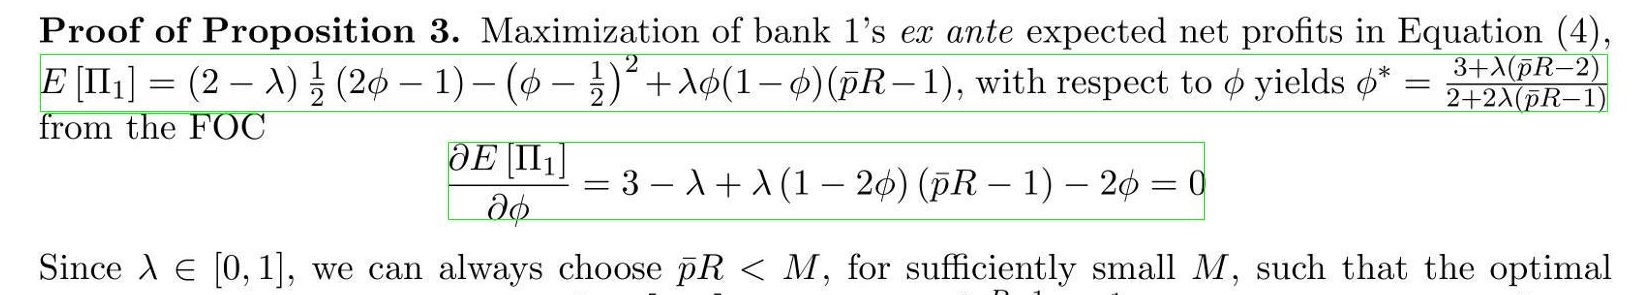
\includegraphics[width=0.4\textwidth]{chem31.jpg}\\ 
  (b)\\ \hline
  \end{tabular} 
 \caption{Examples of segmentation error}
 \label{seg_error}
\end{figure}

% \begin{figure}[h]\center\footnotesize
% \begin{tabular}{|c|}\hline
%  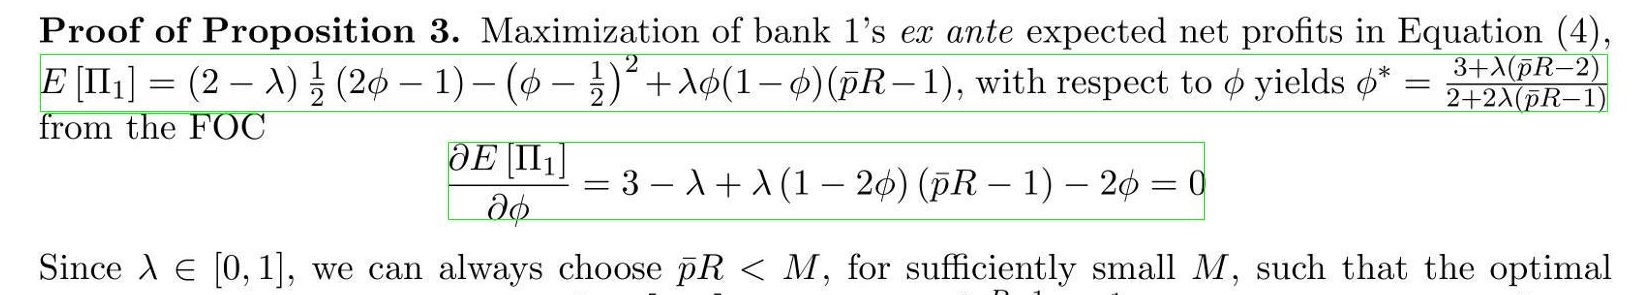
\includegraphics[width=0.4\textwidth]{chem31.png} \\\hline
%  \end{tabular} 
%  \caption{Another example of segmentation error}
%  \label{seg_error1}
% \end{figure}
In a few cases, text lines consisting of embedded expressions are identified as displayed equations 
(see Fig.~\ref{seg_error}(b)), but in those cases the text lines contain more mathematics than normal text.
However, identification of mathematics intensive text lines as mathematical displayed equation is not a severe error. 

 \item Classification error:\\
 In some cases if the operands of a chemical equation have Alkyl or Halide group, 
 they are denoted as R and X respectively. 
 But these symbols are not present in the periodic table.
 Hence, when the substrings from the OCR output are searched in the dictionary, it comes back negative.
 The equation is detected as a non-chemical one. See 4th equation bounded with a green rectangle in Fig.~\ref{cl_error}.  
\begin{figure}[h]\center\footnotesize
\begin{tabular}{|c|}
\hline
 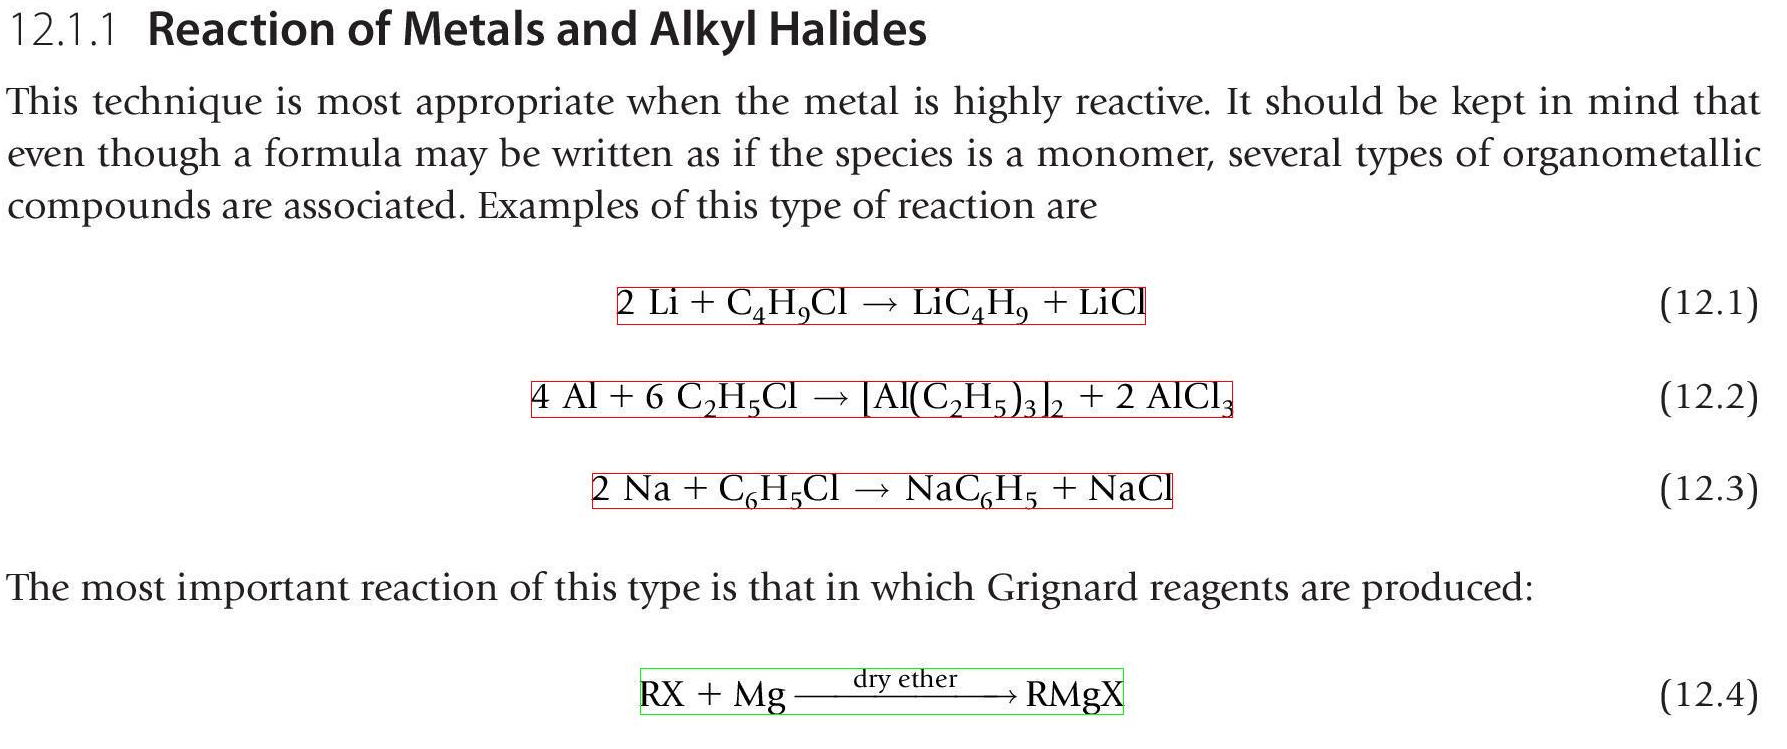
\includegraphics[width=0.42\textwidth]{cbook16.png} \\ \hline
 \end{tabular} 
 \caption{An Example of classification error.}
 \label{cl_error}
\end{figure}
\end{itemize}


\section{Conclusion}
\label{sc_conclu}
We have presented an automated chemical and non-chemical equation segmentation system able to
detect displayed equations of both categories from heterogeneous document images. 
The method is based on detecting operators as +, - and $ \rightarrow$ which are common in both chemical and non-chemical equations,
segmenting the displayed equations and then running them through an open source OCR to classify.
A publicly available database for mathematical documents and scanned images of various chemistry 
books in  both English and Bengali language are used in this study. 
The experimental results demonstrate the efficiency of our proposed method. 
The present work points to several new research avenues to be explored further. 
The over-all performance itself demands further research in this area. Excessive degradation due to aging and
improper digitization of the document images give rise to broken and merged characters which give conflicting output
from the OCR. In the future, design of a better integrated OCR specifically for
chemical equations would be ventured in.
In addition, formation of  ``electron bond matrix"  of a chemical compound in a reaction mentioned in 
the introduction section would be a high-level goal in the future.
\begin{thebibliography}{1}
\bibitem{blostein_97}
 D. Blostein and A. Grabavec.
\newblock {\em ``Recognition of Mathematical Notation'',}
\newblock {\em Handbook of Character Recognition and document Image Analysis}, 557--582, 1997.

\bibitem{chan_2000}
K-F. Chan and D-Y. Yeung.
\newblock {\em``Mathematical Expression Recognition: A Survey''.}
\newblock {\em IJDAR, Vol. 3, no, 1}, 3--15, 2000.

\bibitem{Garain_07}
U. Garain and B. B. Chaudhuri.
\newblock {\em On OCR of Printed mathematical Expressions.}
\newblock {\em ``Digital Document Processing'',Ed. B. B. Chaudhuri, Advances in pattern 
Recognition}, 235--259 , 2007.

\bibitem{fateman_96}
\newblock R. Fateman, T. Tokuyasu, B. Berman, and N. Mitchell.
\newblock {\em ``Optical character recognition and parsing of typeset mathematics'',
Visual Commun. And Image Representation, Vol 7, no 1}, 2--15, 1996.

\bibitem{toumit_99}
\newblock J. Y. Toumit, S. Garcia-Salicetti, and H. Emptoz.
\newblock {\em ``A hierarchical and recursive model of mathematical expressions for
automatic reading of mathematical documents''. In Proc. of
ICDAR}, 116--122, 1999.
 
\bibitem{kacem_01}
\newblock A. Kacem, A. Beliad and M. Ben Ahmed.
\newblock {\em ``Automated Extraction of printed mathematical formulas using fuzzy logic
and propagation of context'', IJDAR, vol.4 no. 2}, 97--108, 2001.

\bibitem{suzuki_03}
\newblock M. Suzuki, F. Tamari, R. Fukuda, S. Uchida and T. Kanahori.
\newblock {\em ``INFTY - An Integrated OCR system for Mathematical Documents'', Proc. of 
ACM Symposium on Document Engineering}, 95--104, 2003.

\bibitem{Garain_09}
\newblock Utpal Garain.
\newblock {\em `` Identification of Mathematical Expressions in Document Images'',
Proc. of ICDAR}, 1340--1344, 2009.

\bibitem{Garain_05}
\newblock Utpal Garain.
\newblock {\em ``Recognition of Printed Handwritten Mathematical Expressions'', Ph.D Thesis,
ISI, Kolkata, India}, 2005.

\bibitem{Garain_01}
\newblock B. B. Chaudhuri and U. Garain.
\newblock {\em ``Extraction of type atyle based meta-information from Imaged
documents'', IJDAR, vol. 3 no. 3}, 138--149, 2001.

\bibitem{jin_03}
\newblock J. Jin, X. Han and Q. Wang.
\newblock {\em ``Mathematical formulas extraction'', Proc. of ICDAR}, 1138--1141, 2003.

\bibitem{drake_05}
\newblock D. M. Drake and H. S. Baird.
\newblock {\em ``Distinguishing mathematical notation from english text
using computational geometry'', Proc. of ICDAR}, 1270--1274, 2005.

\bibitem{guo_07}
\newblock Y.-S. Guo, L. Huang and C.-P. Liu.
\newblock {\em ``A new approach for understanding of structure of printed mathematical
expressions'', Proc. of ICMLC}, 2633--2638, 2007.

\bibitem{liu_13}
\newblock We-Te Chu and Fan liu.
\newblock {\em ``Mathematical formula detection from heterogeneous document
Images'', Proc. of CTAAI}, 140--146, 2013.

\bibitem{skm_07}
S. P. Chowdhury, S. Mandal, A. K. Das, and B. Chanda.
\newblock {\em ``Segmentation of Text and Graphics from Document Images''},
\newblock in {\em Proc. of ICDAR}, 619--623, 2007.

\bibitem{gonzalez92}
R.~C.~Gonzalez and R.~Woods.
\newblock {\em ``Digital Image Processing''}.
\newblock Addision-Wesley, 1992.

\bibitem{skm_06}
S. Mandal, S. P. Chowdhury, A. K. Das, and B. Chanda,
\newblock {\em ``A simple and effective table detection system from Document Images''},
\newblock in {\em Proc. of IJDAR, Vol. 8(2)}, 172--182, 2006.

\end{thebibliography}


\end{document}




\section{Experimental Result}
\label{sc:exp-res}

We have implemented our algorithm in MATLAB 8.3.0.532 (R2014 a) in a PC (Intel core 2 Duo T6500 2.10\,GHz CPU running Windows).
We have tested our algorithm on various digitized documents scanned from different books \cite{mano_book,Pucknell_book}.
 In Fig.~\ref{fig:final}(b), all the symbols are correctly segment out except one resistor which is over segmented.
 Also, one resistor is segmented with an earthing symbol as the gap between resistor and earthing symbol is very small. But all this problem can be solved by a post processing
 during the recognition of the symbol as there is a particular feature of each of these symbols.
 Fig.~\ref{fig:exp1} and Fig.~\ref{fig:exp2} shows another results of our algorithm. 
 In Fig.~\ref{fig:exp2} the arrow shape is also segmented as a symbol.
 
Table~\ref{tab:summary} gives the details of experimental results on 10 images from the datasets of electrical circuit drawings.



\begin{figure}[h]\center\footnotesize
\begin{tabular}{|c|c|}
\hline
 \includegraphics[width=0.23\textwidth]{Image18.png} &
 \includegraphics[width=0.21\textwidth]{final_image18.png} \\
 (a) Input Image &(b) Segmented symbols \\
 \hline
 \end{tabular} 
 \caption{Result of segmentation algorithm.}
 \label{fig:exp1}
\end{figure}



\begin{figure}[h]\center\footnotesize
\begin{tabular}{|c|}
\hline
 \includegraphics[width=0.45\textwidth]{Image33.png} \\
 (a) Input image \\\hline\\
 \includegraphics[width=0.42\textwidth]{final_image33.png} \\ 
 (b) Segmented symbols\\ \hline
 \end{tabular} 
 \caption{Result of segmentation algorithm}
 \label{fig:exp2}
\end{figure}


\begin{table}[h]\center\scriptsize
\caption{ Summary of experimental results}
\begin{tabular}{|l|c|c|c|c|c|}\hline
                   
Image              & No. of   & Correctly & Over     &   Under    & Not\\ 
File               & symbols  & segmented & segmented&  segmented & segmented\\ \hline 
Image1.pbm         &     10   &    9      &  0       &    1       & 0\\ \hline 
Image2.pbm         &     24   &   17      &  4       &    0       & 3 \\ \hline 
Image3.pbm         &     11   &   11      &  0       &    0       & 0   \\ \hline 
Image4.pbm         &     21   &   21      &  0       &    0       & 0     \\ \hline 
Image5.pbm         &     9    &    8      &  0       &    1       & 0   \\ \hline  
Image22.pbm        &     8    &    6      &  2       &    0       & 0   \\\hline
Image30.pbm        &     22   &   19      &  2       &    0       & 0   \\\hline
Image35.pbm        &     17   &   17      &  0       &    0       & 0   \\ \hline 
Image37.pbm        &     12   &   12      &  0       &    0       & 0     \\ \hline
      Total \%     &     0    &   0       &  0       &    0       & 0      \\ \hline
\end{tabular}
\label{tab:summary}
\end{table}
% 
% \begin{figure}[h]\footnotesize
% \begin{tabular}{cc}
%  \includegraphics[width=0.22\textwidth]{Image34.png} &
%  \includegraphics[width=0.22\textwidth]{Image34-text1.png} \\\\
%  (a) Input Image &(b) Text removal\\
%  \includegraphics[width=0.22\textwidth]{Image34-h_line1.png} &
%  \includegraphics[width=0.22\textwidth]{Image34-v_line1.png} \\\\
%  (c) Horizontal line segments &(d) Vertical line segments\\\\
%  \includegraphics[width=0.22\textwidth]{Image34-final-seg.png} &
%  %\includegraphics[width=0.24\textwidth]{Image34-v_line.png} 
%  \\\\\\
%  (e)&(f)\\
%  \end{tabular}
%  \caption{Step by step result of segmentation procedure.}
%  \label{fig:opa}
% \end{figure}

\section{Conclusion}
\label{sc:conclu}

The proposed segmentation algorithm successfully segment all the electrical symbols and finally separate the symbols and the 
connecting wires in the circuit in two different spaces $C$ and $W$. The algorithm is computationally cheaper as it uses the basic
image processing operations like morphology and histogram analysis. The algorithm gives the correct result in case of noisy images and also for the skewed images.
The main advantage is that the algorithm is symbol orientation independent.
The symbols that are closely connected mainly in case of earthing symbols the symbols are not correctly segmented can also be segmented during recognition step in future.

%%%%%%%%%%%%%%%%%%%%%%%%%%%%%%%%%%%%%%%%%%%%%%%%%%%%%%%%%%%%%%%%%%%%%%%%%%%%%%%%%%%%%%%%%%%%%%%%%%%%%%%%%%%%%%%%%%%%%
% \bibliographystyle{abbrv}%{IEEEtran}%{abbrv}%{ieee}
% \bibliography{sym,skm}

\begin{thebibliography}{1}

% 
% \bibitem{Boraie:1997}
% M.~Boraie and A.~Balghonaim.
% \newblock Optical recognition of electrical circuit drawings.
% \newblock In {\em IEEE Pacific Rim Conference Networking}, pp.\,843--846, 1997.
%\bibitem{Garain_07}
%U. Garain and B. B. Chaudhuri. On OCR of Printed mathematical
%Expressions. “Digital Document Processing”,Ed. B. B. Chaudhuri,
%Advances in pattern Recognition, 235–259 , 2007.



\bibitem{cheng_93}
T.~Cheng, J.~Khan, H.~Liu, and D.~Yun.
\newblock A symbol recognition system.
\newblock In {\em Proc. ICDAR}, pp.\,918--921, Oct. 1993.
% 
% \bibitem{das2001a}
% A.~K. Das and B.~Chanda.
% \newblock A fast algorithm for skew detection of document images using  morphology.
% \newblock {\em IJDAR}, 4:109--114, 2001.
\bibitem{blostein_97}
D. Blostein and A. Grabavec
\newblock Recognition of Mathematical Notation.
\newblock {\em Handbook of Character Recognition and document Image Analysis}, 557--582, 1997.
\bibitem{Fukada1984}
Y.~Fukada.
\newblock A primary algorithm for the understanding of logic circuit diagrams.
\newblock {\em Pattern Recognition}, 17:125--134, 1984.

\bibitem{gonzalez92}
R.~C.~Gonzalez and R.~Wood.
\newblock {\em Digital Image Processing}.
\newblock Addision-Wesley, 1992.

\bibitem{groen_85}
F.~C. Groen, A.~C. Sanderson, and J.~F. Schlag.
\newblock Symbol recognition in electrical diagrams using probabilistic graph   matching.
\newblock {\em PRL}, 3(5):343--350, 1985.
% 
% \bibitem{Joseph1989}
% S.~Joseph.
% \newblock Processing of engineering line drawings for automatic input to CAD.
% \newblock {\em Pattern Recognition}, 22(1):1--11, 1989.

\bibitem{kasturi_88}
L.~Fletcher and R.~Kasturi,
\newblock ``A robust algorithm for text string separation from mixed text/graphics images,''
\newblock in {\em IEEE TPAMI}, vol.\,10, pp.\,910--918, 1988.


\bibitem{kim1993ICDAR}
S.~Kim, J.~Suh, and J.~Kim.
\newblock Recognition of logic diagrams by identifying loops and rectilinear polylines.
\newblock In {\em Proc. ICDAR}, pp.\,349--352, 1993.
% 
% \bibitem{Kojima1988ICDAR}
% H.~Kojima and T.~Toida.
% \newblock Online hand-drawn line-figure recognition and its application.
% \newblock In {\em Proc. ICPR}, pp.\,1138--1142, 1988.

\bibitem{mano_book}
M.~Mano.
\newblock {\em Digital Logic and Computer Design}.
\newblock Pearson Prentice Hall, 3rd Ed., 2006.


% \bibitem{Murase1986PR}
% H.~Murase and T.~Wakahara.
% \newblock Online hand-sketched figure recognition.
% \newblock {\em Pattern Recognition}, 19(2):147--160, 1986.

\bibitem{Okazaki:1988}
A.~Okazaki, S.~Tsunekawa, T.~Kondo, K.~Mori, and E.~Kawamoto.
\newblock An automatic circuit diagram reader with loop-structure-based symbol recognition.
\newblock {\em IEEE Trans. PAMI}, 10:331--341, 1988.
% 
\bibitem{otsu79}
N.~Otsu.
\newblock A threshold selection method from gray-level histogram.
\newblock {\em IEEE Trans. SMC}, pp.\,62--66, 1979.


\bibitem{Pucknell_book}
D.~A. Pucknell and K.~Eshraghian.
\newblock {\em Basic VLSI Design}.
\newblock PHI, 3rd Ed., 2000.

\bibitem{skm_07}
S. P. Chowdhury, S. Mandal, A. K. Das, and B. Chanda,
\newblock ``Segmentation of Text and Graphics from Document Images,''
\newblock in {\em ICDAR}, vol.\,2, pp.\,619--623, 2007.

\bibitem{ValoisICDAR2001}
J.-P. Valois, M.~C\^{o}t\'{e}, and M.~Cheriet.
\newblock Online recognition of sketched electrical diagrams.
\newblock {\em ICDAR}, pp.\,460--464, 2001.

\bibitem{Yu1997PAMI}
Y.~Yu, A.~Samal, and S.~Seth.
\newblock A system for recognizing a large class of engineering drawings.
\newblock {\em IEEE Trans. PAMI}, 19(8):868--890, 1997.

%%%%%%%%%%%%%%%%%%%%%%%%%%%%%%%%%%%%%%%%%%%%%%%%%%%%%%%%%%%%%%%%%%%%%%%%%%%%%%%%%%%%%%%%%%%%%%%5
% \bibitem{vijaya2013}
% N.~Priyadharshini, and MS.~Vijaya.
% \newblock Document segmentation and region classification using multilayer perceptron.
% \newblock {\em IJCSI Comp.Sc. issues}, 10(1):193--198, 2013.
% 
% 
% \bibitem{ando2002}
% H.~Ando, T.~Morie, M.~Miyake, M.~Nagata and A.~Iwata.
% \newblock Image Segmentation/Extraction Using Nonlinear Cellular Networks and Their 
% VLSI Implementation Using Pulse-Modulation Techniques.
% \newblock {\em IEICE Trans. Fundamentals}, E85-A(2):381--388, 2002.
%%%%%%%%%%%%%%%%%%%%%%%%%%%%%%%%%%%%%%%%%%%%%%%%%%%%%%%%%%%%%%%%%%%%%%%%%%%%%%%%%%%%%%%%%%%5


\bibitem{kasturi_98}
H.~Luo and R.~Kasturi.
\newblock Improved Directional Morphological Operations for separation of Characters from
Maps/Graphics.
\newblock {\em Springer-Verlag}, pp.\,35--47, 1998.


\bibitem{jain_97}
A. k.~Jain and S.~Bhattacharjee.
\newblock Texture segmentation using gabor filters for automatic document processing.
\newblock {\em Machine Vision and Application}, 5:169--184, 1992.


\bibitem{santanu_07}
L. Fletcher and R. Kasturi,
\newblock Text Extraction and Document Image Segmentation Using Matched Wavelets and MRF Model.
\newblock in {\em IEEE trans. Pattern Recognition}, vol.\,16(8), pp.\,2117--2128, 2007.



\bibitem{chiang_98}
J.~Chiang, S.~Tue, and Y.~Leu.
\newblock A new algorithm for line image vectorization.
\newblock {\em Pattern Recognition}, 12:1541--1549, 1998.


\bibitem{han_94}
C. C.~Han, and K. C.~Fan.
\newblock Skeleton generation of engineering drawings via contour matching.
\newblock {\em Pattern Recognition}, 27(2):261-275, 1994.


\bibitem{pavlidis_86}
T.~Pavlidis.
\newblock A vectorizer and feature extractor for document recognition.
\newblock {\em CVGIP}, 35:111-127, 1986.


\bibitem{song_2000}
J.~Song, F.~Su, C.~Tai, J.~Chen and S.~Cai.
\newblock Line net global vectorization: An algorithm and its performance evaluation.
\newblock In {\em Proc. CVPR}, pp\,383--388, 2000.


\bibitem{tombre_2002}
K.~Tombre, S.~Tabbone, L.~P\'elissier, B.~Lamiroy and P.~Dosch.
\newblock Text/Graphics Separation Revisited.
\newblock In {\em Proc. Fifth IAPR Int’l Workshop Document Analysis Systems}, 2002.


\bibitem{Akindele_1993}
O. T.~Akindele and A.~Belaid.
\newblock Page segmentation by segment tracing.
\newblock In {\em ICDAR}, pp\, 341--344, 1993.


\bibitem{das_98}
A.~K. Das and B.~Chanda.
\newblock Segmentation of text and graphics from document image: A morphological approach.
\newblock {\em ICCLSDP}, pp\, A50--A56, 1998.


\bibitem{fan_94}
K. C.~fan, C. H.~Liu, and Y. K.~Wang.
\newblock Segmentation and classification of mixed text/graphics/image documents.
\newblock {\em PRL}, 15:1201--1209, 1994.


\bibitem{Yu_97}
A. k.~Jain and B.~Yu.
\newblock Page segmentation using document model.
\newblock In {\em Proc. ICDAR}, pp\, 34--38, 1997.


\bibitem{Liu_98}
W.~Liu, and D.~Dori.
\newblock A generic integrated line detection algorithm and its object-process specification.
\newblock {\em CVIU}, 70(3):420--437, 1998.


\bibitem{pavlidis_92}
T.~Pavlidis, and J.~Zhou.
\newblock Page segmentation and classification.
\newblock {\em CVGIP}, 54:484--496, 1992.


\bibitem{wahl_82}
F. M.~Wahl, K. Y.~Wong and R. G.~Casey.
\newblock Block segmentation and text extraction in mixed text/image documents.
\newblock {\em CGIP 20}, pp\, 375--390, 1982.

\end{thebibliography}


 \section*{Appendix}\label{appendix}
 
 
\begin{table}[h]\center\scriptsize
\caption{ Electrical symbols}
\begin{tabular}{|l|cc|}\hline
 {\em Component name}  &\multicolumn{2}{c}{Symbol}\vline \\\hline
Resistor               & \includegraphics[width=0.032\textwidth]{resh.png}     & \includegraphics[width=0.016\textwidth]{resv.png}\\\hline
Variable resistor 	& \includegraphics[width=0.032\textwidth]{resvr.png}    & \includegraphics[width=0.032\textwidth]{resvr1.png}\\\hline
Potentiometer		& \includegraphics[width=0.035\textwidth]{potm.png}     & \\\hline
Capacitor 		& \includegraphics[width=0.015\textwidth]{caph.png}     &\includegraphics[width=0.018\textwidth]{caph1.png}\\\hline
Variable capacitor	& \includegraphics[width=0.02\textwidth]{capvr.png}     &\\\hline
Inductor		& \includegraphics[width=0.04\textwidth]{indh.png}      &\includegraphics[width=0.015\textwidth]{indv.png}\\\hline
Battery	 	        & \includegraphics[width=0.03\textwidth]{bv.png}        &\includegraphics[width=0.026\textwidth]{bh.png}\\\hline
Battery Cell	 	& \includegraphics[width=0.035\textwidth]{bhc.png}      &\includegraphics[width=0.008\textwidth]{bvc.png}\\\hline
AC Voltage Source	& \includegraphics[width=0.032\textwidth]{source_ac.png}&\\\hline
Current Source	 	& \includegraphics[width=0.032\textwidth]{source_cr.png}&\\\hline
Voltage Source		& \includegraphics[width=0.03\textwidth]{source_vl.png}&\\\hline 
Diode	 		& \includegraphics[width=0.032\textwidth]{dio.png}      & \includegraphics[width=0.035\textwidth]{dio1.png}\\\hline
Zener diode		& \includegraphics[width=0.038\textwidth]{dioz1.png}    & \includegraphics[width=0.028\textwidth]{dioz.png}\\\hline
Inverter 		& \includegraphics[width=0.038\textwidth]{Inv.png}      &\\\hline
BJT Transistor 	        & \includegraphics[width=0.022\textwidth]{trn.png}      &\includegraphics[width=0.035\textwidth]{trn1.png}	\\\hline
MOS transistor 	        & \includegraphics[width=0.035\textwidth]{trnm.png}     & \includegraphics[width=0.034\textwidth]{nmos-trn.png}\includegraphics[width=0.03\textwidth]{mosfet.png}\\\hline
Transformer		& \includegraphics[width=0.04\textwidth]{trfh.png}      &\includegraphics[width=0.025\textwidth]{trfv.png}\\\hline
Operational amplifier  & \includegraphics[width=0.028\textwidth]{opa.png}      &\\\hline
Earth ground   	        & \includegraphics[width=0.035\textwidth]{earth.png}    &\\\hline
Common ground   	& \includegraphics[width=0.035\textwidth]{earth1.png}   &\\\hline
Switch			& \includegraphics[width=0.035\textwidth]{switch1.png}  & \includegraphics[width=0.035\textwidth]{switch2.png}\\\hline
\end{tabular}
\label{tab:symbol}
\end{table}




\end{document}
